\documentclass[10pt,twoside]{article}

% =====================================================================
% 1. PREÂMBULO E CORES
% =====================================================================
\usepackage[brazilian]{babel}
\usepackage[margin=2cm, top=2.5cm, bottom=2.5cm, headheight=17pt, footskip=30pt]{geometry} 
\usepackage{setspace}
\setstretch{1.15}

\setlength{\parindent}{1.25em}
\setlength{\parskip}{0pt}
\setlength{\columnsep}{1cm}

% Ativação da fonte Verdana 
\usepackage{fontspec}
\setmainfont{VERDANA.TTF}[
    BoldFont = VERDANAB.TTF,
    ItalicFont = VERDANAI.TTF,
    BoldItalicFont = VERDANAZ.TTF
]
\usepackage{microtype}

\usepackage{amsmath, amsfonts, amssymb}
\usepackage{booktabs, tabularx, graphicx}
\usepackage{xcolor, tcolorbox}
\usepackage{ccicons} 
\usepackage{indentfirst}
\usepackage{ragged2e}
\usepackage{colortbl}
\usepackage{array}
\usepackage{enumitem}

\usepackage{unicode-math}
\setmathfont{Latin Modern Math}

% Paleta de cores oficial da REPA
\definecolor{REPABLUE}{RGB}{0, 32, 96}     
\definecolor{repabg}{RGB}{222, 234, 246}   
\definecolor{orcidgreen}{RGB}{166, 206, 57}
\definecolor{ccgray}{RGB}{160, 160, 160}

% Configuração dos Títulos das Seções
\usepackage{titlesec}
\titleformat{\section}{\normalfont\fontsize{11}{13}\bfseries\color{REPABLUE}\MakeUppercase}{\thesection}{1em}{} 
\titleformat{\subsection}{\normalfont\fontsize{11}{13}\bfseries\color{REPABLUE}}{\thesubsection}{1em}{} 
\titleformat{\subsubsection}{\normalfont\fontsize{11}{13}\bfseries\color{REPABLUE}}{\thesubsubsection}{1em}{} 

\addto\captionsbrazilian{
    \renewcommand{\refname}{REFERÊNCIAS}
}

% Pacote para links
\usepackage[hidelinks]{hyperref}
\hypersetup{
    colorlinks=true,
    citecolor=REPABLUE,
    linkcolor=REPABLUE,
    urlcolor=blue
}

% =====================================================================
% CONFIGURAÇÃO DE CABEÇALHOS E RODAPÉS
% =====================================================================
\usepackage{fancyhdr}
\pagestyle{fancy}
\fancyhf{} 

\renewcommand{\headrule}{{\color{REPABLUE}\hrule width\headwidth height 1pt}}
\renewcommand{\footrule}{{\color{REPABLUE}\hrule width\headwidth height 1pt}}

% Páginas Pares (Esquerda)
\fancyhead[RE]{\small\textcolor{REPABLUE}{Mineração de Séries Temporais para Previsão da Inflação}}
\fancyfoot[LE]{\small\textcolor{REPABLUE}{\thepage}}
\fancyfoot[RE]{
\includegraphics[height=18pt]{logo_cc.png}\hspace{1.5cm}} 

% Páginas Ímpares (Direita)
\fancyhead[RO]{\small\textcolor{REPABLUE}{Revista de Engenharia e Pesquisa Aplicada, v. xx, n. xx, 2026.}}
\fancyfoot[LO]{\small\textcolor{REPABLUE}{\thepage}}
\fancyfoot[RO]{\small\textcolor{REPABLUE}{DOI: 10.xxxx/xxxx}}

% --- ESTILO DA PRIMEIRA PÁGINA (Limpa) ---
\fancypagestyle{primeirapagina}{
  \fancyhf{} 
  \renewcommand{\headrule}{} 
  \renewcommand{\footrule}{} 
}

% =====================================================================
% INÍCIO DO DOCUMENTO
% =====================================================================
\begin{document}

\thispagestyle{primeirapagina}

% =====================================================================
% 2. CABEÇALHO, AUTORES E RESUMO (PÁGINA 1)
% =====================================================================
\begingroup

\raggedright
\vspace*{-0.6cm} 
{\color{REPABLUE}\hrule height 0.6pt} 
\vspace{0.35cm} 

{\fontsize{16}{18}\selectfont\bfseries\textcolor{REPABLUE}{Mineração de Séries Temporais para Previsão da Inflação: Arquitetura Híbrida Multivariada e Otimização Bioinspirada de Atributos} \par} 
\vspace{0.40cm} 

{\fontsize{11}{13}\selectfont\itshape\textcolor{REPABLUE}{Time Series Mining for Inflation Forecasting: Multivariate Hybrid Architecture and Bio-Inspired Feature Optimization} \par} 
\vspace{0.70cm} 

\begin{tabularx}{\textwidth}{
    >{\raggedright\arraybackslash}X
    >{\raggedright\arraybackslash}X
    >{\raggedright\arraybackslash}X
    >{\raggedright\arraybackslash}X
}
  {\fontsize{9.5}{11.5}\selectfont\bfseries Bruno Protásio$} &
  {\fontsize{9.5}{11.5}\selectfont\bfseries Daniel Meneses$} &
  {\fontsize{9.5}{11.5}\selectfont\bfseries Marcus Vinicius$} &
  {\fontsize{9.5}{11.5}\selectfont\bfseries Vinicyus Emanuel$} \[-0.05cm]

  {\fontsize{7.5}{9.5}\selectfont\textcolor{teal}{orcid.org/xxxx-xxxx-xxxx-xxxx}} &
  {\fontsize{7.5}{9.5}\selectfont\textcolor{teal}{orcid.org/xxxx-xxxx-xxxx-xxxx}} &
  {\fontsize{7.5}{9.5}\selectfont\textcolor{teal}{orcid.org/xxxx-xxxx-xxxx-xxxx}} &
  {\fontsize{7.5}{9.5}\selectfont\textcolor{teal}{orcid.org/xxxx-xxxx-xxxx-xxxx}}
\end{tabularx}
\vspace{0.55cm} 

% BLOCO INFERIOR (Metadados à esquerda e Box de Resumo à direita)
\noindent
\makebox[\textwidth][l]{%
\begin{minipage}[t][15.8cm][t]{0.32\textwidth}
  \raggedright 
  \fontsize{7.5}{9.5}\selectfont 
  \vspace{0.25cm} 
  
  \noindent  Politécnica de Pernambuco, Universidade de Pernambuco (POLI-UPE), Recife, Brasil. \
  Docente Orientador: Prof. Dr. Alexandre Maciel. \
  E-mails: \href{mailto:xxxx@xxxx.com}{\underline{xxxx@xxxx.com}}. \[0.25cm]
  \noindent \textcolor{REPABLUE}{\textbf{Artigo recebido em:}} 15/09/2026 \
  \textcolor{REPABLUE}{\textbf{Artigo aceito em:}} 14/10/2026 \[0.35cm]
  \noindent \textcolor{REPABLUE}{\textbf{DOI:}} 10.xxxx/xxxx \[0.35cm]
  \noindent \textcolor{REPABLUE}{Esta obra apresenta Licença Creative Commons Atribuição-Não Comercial 4.0 Internacional.} \[0.35cm]
  \noindent \textcolor{REPABLUE}{\textbf{Como citar este artigo pela NBR 6023/2018:}} PROTÁSIO, B.; MENESES, D.; VINICIUS, M.; EMANUEL, V. Mineração de Séries Temporais para Previsão da Inflação: Arquitetura Híbrida Multivariada e Otimização Bioinspirada de Atributos. \textbf{Revista de Engenharia e Pesquisa Aplicada}, Recife, v. xx, n. xx, p. xx-xx, 2026. DOI: 10.xxxx/xxxx.
\end{minipage}%
\hspace{0.2cm}%
\textcolor{REPABLUE}{\vrule width 2.5pt} % Linha Azul Vertical
\hspace{0.2cm}%
\begin{minipage}[t][15.8cm][t]{0.68\textwidth}
  \vspace{0pt} 
  \begin{tcolorbox}[
    colback=repabg,
    colframe=repabg,
    arc=0pt,
    outer arc=0pt,
    left=2.5mm,
    right=2.5mm,
    top=3.5mm,
    bottom=2.5mm,
    height=15.8cm
]
    \fontsize{9}{11}\selectfont
    \textcolor{REPABLUE}{\textbf{RESUMO}} \[0.2cm]
    A dinâmica da inflação no Brasil caracteriza-se por uma complexa interação entre inércia contratual e vulnerabilidade a choques macroeconômicos exógenos. Este trabalho investiga a fronteira preditiva do Índice Nacional de Preços ao Consumidor Amplo (IPCA) sob a ótica da Mineração de Dados e Engenharia da Computação. O objetivo central consiste em desenvolver uma arquitetura híbrida multivariada combinando modelagem autoregressiva linear da inércia estocástica e regressores de \textit{machine learning} alimentados por seleção bioinspirada de atributos (\textit{Feature Selection} via Algoritmos Genéticos e PSO). Na presente etapa, estruturou-se um \textit{pipeline} computacional rigoroso de coleta, saneamento, engenharia de atributos e análise exploratória descritiva de um painel de 29 variáveis macroeconômicas extraídas do Banco Central do Brasil, cobrindo o período de 2012 a 2026 (174 meses contínuos). Os métodos empregados englobam padronização temporal \textit{Month-Start}, saneamento de zeros contábeis estruturais, imputação temporal sem vazamento de dados (\textit{zero data leakage}), codificação trigonométrica da sazonalidade e discretização paramétrica dos regimes inflacionários (Deflação, Meta e Alta). A análise descritiva revelou assimetria positiva (+0,53), concentração da mediana em 0,38\% a.m. e presença de cinco \textit{outliers} estruturais associados a choques de oferta e rupturas de cadeias globais de suprimentos. Os resultados estabelecem uma base saneada de alta integridade, fornecendo o arcabouço empírico indispensável para a subsequente calibração dos modelos híbridos e algoritmos de otimização. \[0.3cm]
    \textcolor{REPABLUE}{\textbf{PALAVRAS-CHAVE:}} Mineração de Séries Temporais; Previsão da Inflação; IPCA; Engenharia de Atributos; Econometria Preditiva; \[0.5cm]
    \textcolor{REPABLUE}{\textbf{ABSTRACT}} \[0.2cm]
    \textit{Inflation dynamics in Brazil are characterized by a complex interplay between contractual inertia and vulnerability to exogenous macroeconomic shocks. This study investigates the predictive frontier of the Broad National Consumer Price Index (IPCA) from a Data Mining and Computer Engineering perspective. The main objective of the research is to develop a multivariate hybrid predictive architecture combining linear autoregressive modeling of stochastic inertia with machine learning regressors driven by bio-inspired feature selection (Genetic Algorithms and PSO). In this phase, a rigorous computational pipeline was established for data extraction, cleaning, feature engineering, and exploratory descriptive analysis across 29 macroeconomic variables sourced from the Central Bank of Brazil, spanning from 2012 to 2026 (174 continuous months). Implemented methods encompass Month-Start temporal standardization, structural accounting zero cleansing, leakage-free causal imputation (zero data leakage), cyclical trigonometric seasonal encoding, and parametric discretization of inflation regimes (Deflation, Target, and High). Descriptive analysis revealed positive skewness (+0.53), a median concentration of 0.38\% per month, and five structural outliers linked to supply shocks and global supply chain disruptions. These findings establish a sanitized, high-integrity dataset, providing the empirical foundation required for the subsequent calibration of hybrid predictive models and optimization algorithms.} \[0.3cm]
    \textcolor{REPABLUE}{\textbf{KEY-WORDS:}} \textit{Time Series Mining; Inflation Forecasting; IPCA; Feature Engineering; Predictive Econometrics;}
  \end{tcolorbox}
\end{minipage}%
}

\vspace{0.25cm}
\noindent
\makebox[\textwidth][l]{%
    
\includegraphics[width=6.0cm]{logo_repa.png}%
}

\endgroup

\clearpage
\twocolumn
\justifying

% =====================================================================
% 3. CORPO DO ARTIGO
% =====================================================================

\section{INTRODUÇÃO}

A estabilidade de preços constitui o alicerce fundamental do planejamento econômico, da preservação da renda do trabalho e da alocação eficiente de recursos produtivos em economias em desenvolvimento \cite{ref4, ref16}. No Brasil, a trajetória do Índice Nacional de Preços ao Consumidor Amplo (IPCA), calculado mensalmente pelo Instituto Brasileiro de Geografia e Estatística (IBGE), é determinada pela constante fricção entre a persistência inercial dos contratos e a exposição recorrente a choques de oferta exógenos, tais como oscilações cambiais e quebras na cadeia produtiva \cite{ref5, ref10, ref14}. A literatura preditiva tradicional apoiou-se predominantemente em formulações autorregressivas univariadas, as quais, embora eficazes na captura da inércia estocástica e da sazonalidade, mostram-se lentas na resposta a descontinuidades e perturbações externas \cite{ref1, ref9}. Em contrapartida, abordagens multivariadas fundamentadas em grandes painéis informacionais enfrentam riscos severos de ruído amostral, multicolinearidade e sobreajuste (\textit{overfitting}) \cite{ref6, ref14}.

Diante desse cenário, este projeto de pesquisa tem como objetivo central conceber e validar uma arquitetura híbrida multivariada para a previsão do IPCA, integrando a modelagem da inércia estocástica por processos lineares autorregressivos (ARIMAX) à absorção de choques exógenos residuais não lineares mediante algoritmos de \textit{machine learning} (\textit{Random Forest}) com seleção bioinspirada de atributos (\textit{Feature Selection} via Algoritmos Genéticos e PSO) \cite{ref7, ref8, ref11, ref18}. A relevância aplicada dessa abordagem estrutura-se em três vertentes diretas \cite{ref2, ref12}:
\begin{itemize}[leftmargin=1.5em]
    \item \textbf{Governança Pública e Macroeconômica:} Redução de assimetrias informacionais para a antecipação de pressões de custos antes de sua disseminação na economia, auxiliando na ancoragem das expectativas dos agentes \cite{ref2, ref3};
    \item \textbf{Mercado Financeiro e Atividade Corporativa:} Apoio tempestivo ao planejamento orçamentário empresarial, gestão de risco de tesouraria e correta precificação de contratos e ativos indexados à inflação (como debêntures e títulos NTN-B) \cite{ref12, ref17};
    \item \textbf{Engenharia da Computação e Mineração de Dados:} Consolidação de um ambiente metodológico rigoroso de mineração em séries temporais complexas, solucionando desafios práticos de sincronização multivariada e prevenção de viés preditivo (\textit{zero data leakage}) \cite{ref7, ref14}.
\end{itemize}

No escopo da presente etapa, o foco consiste na formalização conceitual do problema, na estruturação do protocolo interdisciplinar e na implementação do \textit{pipeline} integral de coleta, saneamento, engenharia de atributos e análise exploratória de um painel de 29 variáveis macroeconômicas oficiais (174 meses contínuos, de 2012 a 2026), preparando a base empírica para as etapas posteriores de otimização e calibração preditiva \cite{ref6, ref10}.

\subsection{Descrição do Problema}
O desafio central de modelagem reside em arbitrar entre a inércia temporal e a sensibilidade a choques macroeconômicos externos \cite{ref1, ref6}:
\begin{enumerate}[leftmargin=1.5em]
    \item \textbf{A Hipótese Univariada:} Postula que a inércia inflacionária — sustentada por indexação contratual e rigidez de preços — domina a trajetória da série, de modo que modelos autorregressivos simples superariam formulações complexas que demandam estimativas de terceiros \cite{ref1, ref5};
    \item \textbf{A Hipótese Multivariada:} Postula que indicadores antecedentes de preços no atacado, custos de transporte, cotação do dólar e nível de atividade agregada emitem sinais preditivos antecipados que o histórico isolado do índice de inflação é incapaz de capturar a tempo \cite{ref6, ref14}.
\end{enumerate}

O problema concreto investigado consiste em responder se o enriquecimento do espaço de atributos por meio de séries temporais exógenas selecionadas por algoritmos bioinspirados reduz o erro de generalização em horizontes de 1 a 12 meses à frente em comparação aos modelos clássicos puramente autorregressivos \cite{ref8, ref11, ref18}.

\subsection{Objetivos do Projeto}
\subsubsection{Objetivo Geral da Etapa Atual}
Estruturar o arcabouço computacional e conceitual do projeto, formalizando a parceria com os especialistas de domínio (economistas), delimitando a base de dados longitudinal mensal (2012–2026) e executando o saneamento e a análise descritiva dos atributos \cite{ref7, ref10}.

\subsubsection{Objetivos Específicos do Escopo Atual}
\begin{itemize}[leftmargin=1.5em]
    \item Definir o protocolo de governança interdisciplinar com os especialistas de domínio econômico \cite{ref2, ref14};
    \item Coletar e consolidar 29 variáveis macroeconômicas via API oficial do SGS/BACEN (174 observações mensais contínuas) \cite{ref2, ref10};
    \item Desenvolver e executar rotinas de tratamento de zeros estruturais, sincronização de periodicidades e imputação de valores ausentes sem vazamento de informação temporal (\textit{zero data leakage}) \cite{ref7, ref14};
    \item Realizar a análise exploratória e descritiva dos atributos numérico (IPCA) e nominal derivado (Regimes de Inflação), caracterizando medidas de tendência central, dispersão, assimetria e presença de \textit{outliers} \cite{ref7, ref10};
    \item Estruturar o dicionário de dados final da base consolidada pré-processada \cite{ref2, ref15}.
\end{itemize}

\subsection{Justificativa Metodológica e Aplicada}
Projetos preditivos em econometria aplicada frequentemente falham devido à desconexão entre a sofisticação algorítmica e a realidade operacional das variáveis \cite{ref6, ref12}. A elaboração de um \textit{pipeline} robusto de mineração de dados mitiga riscos de vazamento de dados (\textit{look-ahead bias}), reduz redundâncias colineares e garante que a posterior aplicação de técnicas de inteligência artificial repouse sobre bases empiricamente consistentes \cite{ref6, ref7, ref14}.

\subsection{Delimitação do Escopo e Escopo Negativo}
Em estrita conformidade com o cronograma metodológico da disciplina de Mineração de Dados da POLI-UPE \cite{ref7, ref15}:
\begin{itemize}[leftmargin=1.5em]
    \item \textbf{Não faz parte desta entrega:} O treinamento, teste, validação cruzada temporal ou ajuste de hiperparâmetros de modelos preditivos (ARIMAX, \textit{Random Forest} ou Redes Neurais) \cite{ref1, ref14, ref18};
    \item \textbf{Não faz parte desta entrega:} A execução dos algoritmos bioinspirados de seleção de atributos (Algoritmos Genéticos e Otimização por Enxame de Partículas - PSO) \cite{ref8, ref11};
    \item \textbf{Não faz parte desta entrega:} A comparação de métricas preditivas de acurácia (RMSE, MAE, MAPE) e a disponibilização de interface final para usuários \cite{ref6, ref15}.
\end{itemize}

% =====================================================================
\section{FUNDAMENTAÇÃO TEÓRICA}
% =====================================================================

\subsection{Contexto Macroeconômico: Dinâmica da Inflação e Atuação do BACEN}
Compreender a dinâmica da inflação requer o conhecimento dos canais econômicos que conectam as decisões de política monetária ao índice de preços ao consumidor \cite{ref4, ref13}:

\textbf{O que é a Inflação na Prática?} A inflação corresponde ao aumento generalizado e contínuo do nível de preços de bens e serviços de uma economia ao longo do tempo, acarretando a perda sistemática do poder aquisitivo da moeda nacional \cite{ref4, ref13}.

\textbf{Como o IPCA Mede Essa Realidade?} O IPCA, calculado pelo IBGE desde 1979 e índice oficial do regime de metas desde 1999, afere o consumo pessoal de famílias com rendimento mensal entre 1 e 40 salários mínimos residentes em áreas urbanas de 16 regiões geográficas do país \cite{ref10}. Sua cesta abrange mais de 400 subitens agrupados em 9 grupos ponderados pela Pesquisa de Orçamentos Familiares (POF) \cite{ref10}.

\textbf{Os Três Grandes Motores da Inflação Brasileira:}
\begin{enumerate}[leftmargin=1.5em]
    \item \textbf{Inflação de Custos (Choques de Oferta):} Disparada pela elevação nos custos de insumos essenciais, como combustíveis fósseis, energia elétrica e tarifas logísticas, além do repasse da depreciação cambial (\textit{pass-through}) sobre produtos importados \cite{ref4, ref13};
    \item \textbf{Inflação de Demanda:} Decorrente de pressões em que a demanda agregada por bens e serviços suplanta a capacidade produtiva instalada \cite{ref4, ref13};
    \item \textbf{Inflação Inercial:} Mecanismo de autoperpetuação psicológica e institucional gerado pela indexação formal e informal da economia (aluguéis, salários, tarifas públicas), no qual a inflação passada é compulsoriamente projetada no presente \cite{ref5, ref16}.
\end{enumerate}

\textbf{O Banco Central do Brasil e o 'Termostato' da Política Monetária:} A dinâmica da inflação conecta-se à arquitetura do Sistema Financeiro Nacional, onde o Conselho Monetário Nacional (CMN) estipula as metas anuais e o Banco Central do Brasil (BACEN) opera a taxa básica de juros (Selic) como mecanismo de estabilização \cite{ref2, ref3}. Quando o índice se desvia do centro da meta, o Comitê de Política Monetária (COPOM) eleva a Selic para desaquecer o consumo \cite{ref3, ref17}. O ponto crítico reside na existência de defasagens temporais de transmissão (\textit{transmission lags}), que demandam entre 6 e 12 meses (dois a quatro trimestres) para produzir efeitos plenos sobre o consumo e investimentos, impondo a necessidade de modelos preditivos tempestivos \cite{ref3, ref17}.

\subsection{Mineração de Dados em Séries Temporais e Fundamentação do Agrupamento Hierárquico (Critério de Ward)}
A Mineração de Dados em Séries Temporais (\textit{Time Series Data Mining}) visa descobrir padrões estruturais, tendências latentes e dependências dinâmicas em dados sequenciais indexados cronologicamente \cite{ref7, ref9}. Ao contrário de observações tabulares padrão, séries temporais violam a premissa de observações independentes e identicamente distribuídas (i.i.d.), exigindo tratamento rigoroso de não estacionariedade, quebras estruturais e ordenação temporal \cite{ref7, ref9}. No contexto da inflação brasileira, a identificação de regimes latentes — tanto sazonais intra-anuais quanto macroeconômicos plurianuais — demanda técnicas de aprendizado não supervisionado (\textit{unsupervised learning}) capazes de segmentar períodos históricos sem impor rótulos arbitrários \textit{a priori}.

Dentre as famílias de algoritmos de agrupamento (\textit{clustering}), selecionou-se o \textbf{Agrupamento Hierárquico Aglomerativo baseado no Critério de Mínima Variância de Ward} (\textit{Ward's Hierarchical Agglomerative Clustering}) \cite{ref19}. Enquanto métodos particionais clássicos como o $K$-Means dependem de sementes estocásticas aleatórias de inicialização e assumem partições estritamente hiper-esféricas de variâncias homogêneas, o método de Ward constrói uma árvore hierárquica determinística (\textit{dendrograma}), permitindo inspecionar visual e analiticamente a distância de corte ótima e a estrutura aninhada dos regimes temporais \cite{ref7, ref19}.

\subsubsection{Formulação Matemática do Critério de Mínima Variância de Ward}
O método de Ward opera sob uma estratégia aglomerativa \textit{bottom-up}: inicia-se com $N$ clusters unitários e, a cada iteração $t$, fundem-se iterativamente os dois clusters que proporcionam o \textbf{menor incremento na soma total dos quadrados dos desvios intra-cluster} (\textit{Error Sum of Squares} -- $ESS$) \cite{ref19}. 

Para um agrupamento $C_k$ contendo $n_k$ vetores de atributos $x_i \in \mathbb{R}^p$ e centróide $\bar{x}_k = \frac{1}{n_k} \sum_{x_i \in C_k} x_i$, a variância intra-cluster ($ESS_k$) é formalmente definida como:
\begin{equation}
ESS_k = \sum_{x_i \in C_k} ||x_i - \bar{x}_k||^2
\end{equation}

A função objetivo global para uma partição em $K$ grupos consiste na minimização do somatório das variâncias internas:
\begin{equation}
ESS_{\text{Total}} = \sum_{k=1}^K ESS_k = \sum_{k=1}^K \sum_{x_i \in C_k} ||x_i - \bar{x}_k||^2
\end{equation}

Ao avaliar a união de dois clusters arbitrários $A$ e $B$ com tamanhos $n_A$ e $n_B$ e centróides $\bar{x}_A$ e $\bar{x}_B$, o acréscimo de variância $\Delta ESS_{AB}$ gerado pela fusão corresponde à distância euclidiana ponderada entre seus centróides \cite{ref19}:
\begin{equation}
\Delta ESS_{AB} = ESS_{A \cup B} - (ESS_A + ESS_B) = \frac{n_A \cdot n_B}{n_A + n_B} ||\bar{x}_A - \bar{x}_B||^2
\end{equation}

A cada passo aglomerativo, o algoritmo seleciona o par ótimo $(A^*, B^*)$ que satisfaz o critério de variância mínima:
\begin{equation}
(A^*, B^*) = \arg\min_{A, B} \Delta ESS_{AB}
\end{equation}

\subsubsection{Recorrência de Lance-Williams e Propriedades para Séries Temporais}
A atualização computacional da matriz de dissimilaridades entre o novo cluster fundido $(A \cup B)$ e qualquer outro cluster remanescente $C$ é governada pela equação de recorrência generalizada de Lance-Williams \cite{ref20}:
\begin{equation}
D(A \cup B, C) = \alpha_A D(A, C) + \alpha_B D(B, C) + \beta D(A, B) + \gamma |D(A, C) - D(B, C)|
\end{equation}
onde para o método de Ward os coeficientes são $\alpha_A = \frac{n_A + n_C}{n_A + n_B + n_C}$, $\alpha_B = \frac{n_B + n_C}{n_A + n_B + n_C}$, $\beta = -\frac{n_C}{n_A + n_B + n_C}$ e $\gamma = 0$ \cite{ref7, ref20}. Essa formulação confere determinismo estrito, preservação de assimetrias estruturais de frequência e auditabilidade topológica.

\subsection{Trabalhos Relacionados e Análise de Diferenciais}
A literatura contemporânea divide-se em três grandes linhagens metodológicas:
\begin{enumerate}[leftmargin=1.5em]
    \item \textbf{Modelagem Paramétrica Box-Jenkins:} A abordagem clássica ARIMA/SARIMA captura a inércia estocástica e a sazonalidade, mas parte de hipóteses rígidas de linearidade e não responde tempestivamente a choques de oferta exógenos \cite{ref1, ref9};
    \item \textbf{Vetores Autorregressivos (VAR/VECM):} Modela interdependências macroeconômicas simultâneas, porém sofre severamente com a 'maldição da dimensionalidade' quando o número de defasagens e variáveis aumenta \cite{ref4};
    \item \textbf{Machine Learning Multivariado de Alta Dimensionalidade:} Modelos como Lasso, Elastic Net e \textit{Random Forest} exploram amplos painéis econômicos \cite{ref6, ref14}, mas correm o risco de ignorar a ancoragem da inércia autorregressiva estrutural se aplicados diretamente sem modelagem híbrida de resíduos \cite{ref6, ref14, ref18}.
\end{enumerate}

A Tabela 1 sintetiza o posicionamento metodológico e os diferenciais da arquitetura adotada neste projeto.

\begin{table*}[t]
\centering
{\raggedright \fontsize{10}{12}\selectfont \textbf{\textcolor{REPABLUE}{Tabela 1 -}} Matriz Comparativa de Trabalhos Relacionados e Diferenciais Metodológicos do Projeto\par}
\vspace{0.2cm}
\arrayrulecolor{REPABLUE}
\setlength{\arrayrulewidth}{1pt}
\renewcommand{\arraystretch}{1.2}
\fontsize{7.5}{9.5}\selectfont
\begin{tabularx}{\textwidth}{p{0.18\textwidth}X X X >{\columncolor{repabg}}X}
\hline
\textbf{Critério / Dimensão} & \textbf{Abordagem Univariada (Box-Jenkins) \cite{ref1}} & \textbf{Modelos Econométricos (VAR / VEC) \cite{ref4}} & \textbf{Machine Learning Multivariado \cite{ref6, ref14}} & \textbf{Arquitetura Híbrida Proposta (Este Projeto)} \
\hline
\textbf{Captura da Inércia Inflacionária} & Ótima (polinômios autorregressivos puros). & Moderada (limitada pelo número de defasagens). & Baixa a moderada (não modela a dependência pura). & \textbf{Ótima (componente ARIMAX dedicado à inércia estocástica).} \
\hline
\textbf{Tratamento de Choques Não Lineares} & Incapaz de modelar quebras estruturais ou choques exógenos. & Modela não linearidades endógenas, mas cego a choques pontuais. & Captura interações não lineares, negligencia a inércia pura. & \textbf{ARIMAX ancora a inércia e a \textit{Random Forest} absorve os choques residuais.} \
\hline
\textbf{Espaço de Atributos e Seleção} & Nulo (apenas defasagens da própria série temporal). & Pequeno porte (3 a 6 variáveis para evitar sobreparametrização). & Amplo painel (50 a 100 séries via regularização Lasso/Ridge). & \textbf{29 covariáveis selecionadas via Algoritmos Genéticos e PSO bioinspirados.} \
\hline
\textbf{Prevenção de Vazamento Temporal} & Triviais pela natureza univariada do processo. & Moderada, suscetível a revisões metodológicas de séries. & Crítica: requer validação em janelas expansivas ou deslizantes. & \textbf{Protocolo rigoroso de janelas deslizantes (\textit{rolling windows}).} \
\hline
\textbf{Interpretabilidade e Domínio} & Alta interpretabilidade estatística formal. & Alta coerência conceitual com funções impulso-resposta. & Caixa-preta (dificuldade de audição por formuladores). & \textbf{Alta transparência: decomposição em inércia linear + resíduo não linear.} \
\hline
\end{tabularx}
\vspace{0.1cm}
{\raggedright \fontsize{8}{10}\selectfont \textbf{Fonte:} Elaboração própria com base na revisão de literatura metodológica (2026).\par}
\end{table*}

% =====================================================================
\section{MATERIAIS E MÉTODOS}
% =====================================================================

A metodologia adotada para o desenvolvimento deste trabalho articula-se em quatro fases fundamentais, estruturadas sob um fluxo estrito de engenharia de dados e modelagem estatística. A Figura 1 ilustra o fluxograma metodológico global do projeto, evidenciando as etapas executadas no presente marco e as atividades planejadas para a fase subsequente.

\begin{figure*}[t]
    \centering
    {\fontsize{10}{12}\selectfont \textbf{Figura 1} – Fluxograma Metodológico do \textit{Pipeline} de Mineração de Dados}\[0.2cm]
    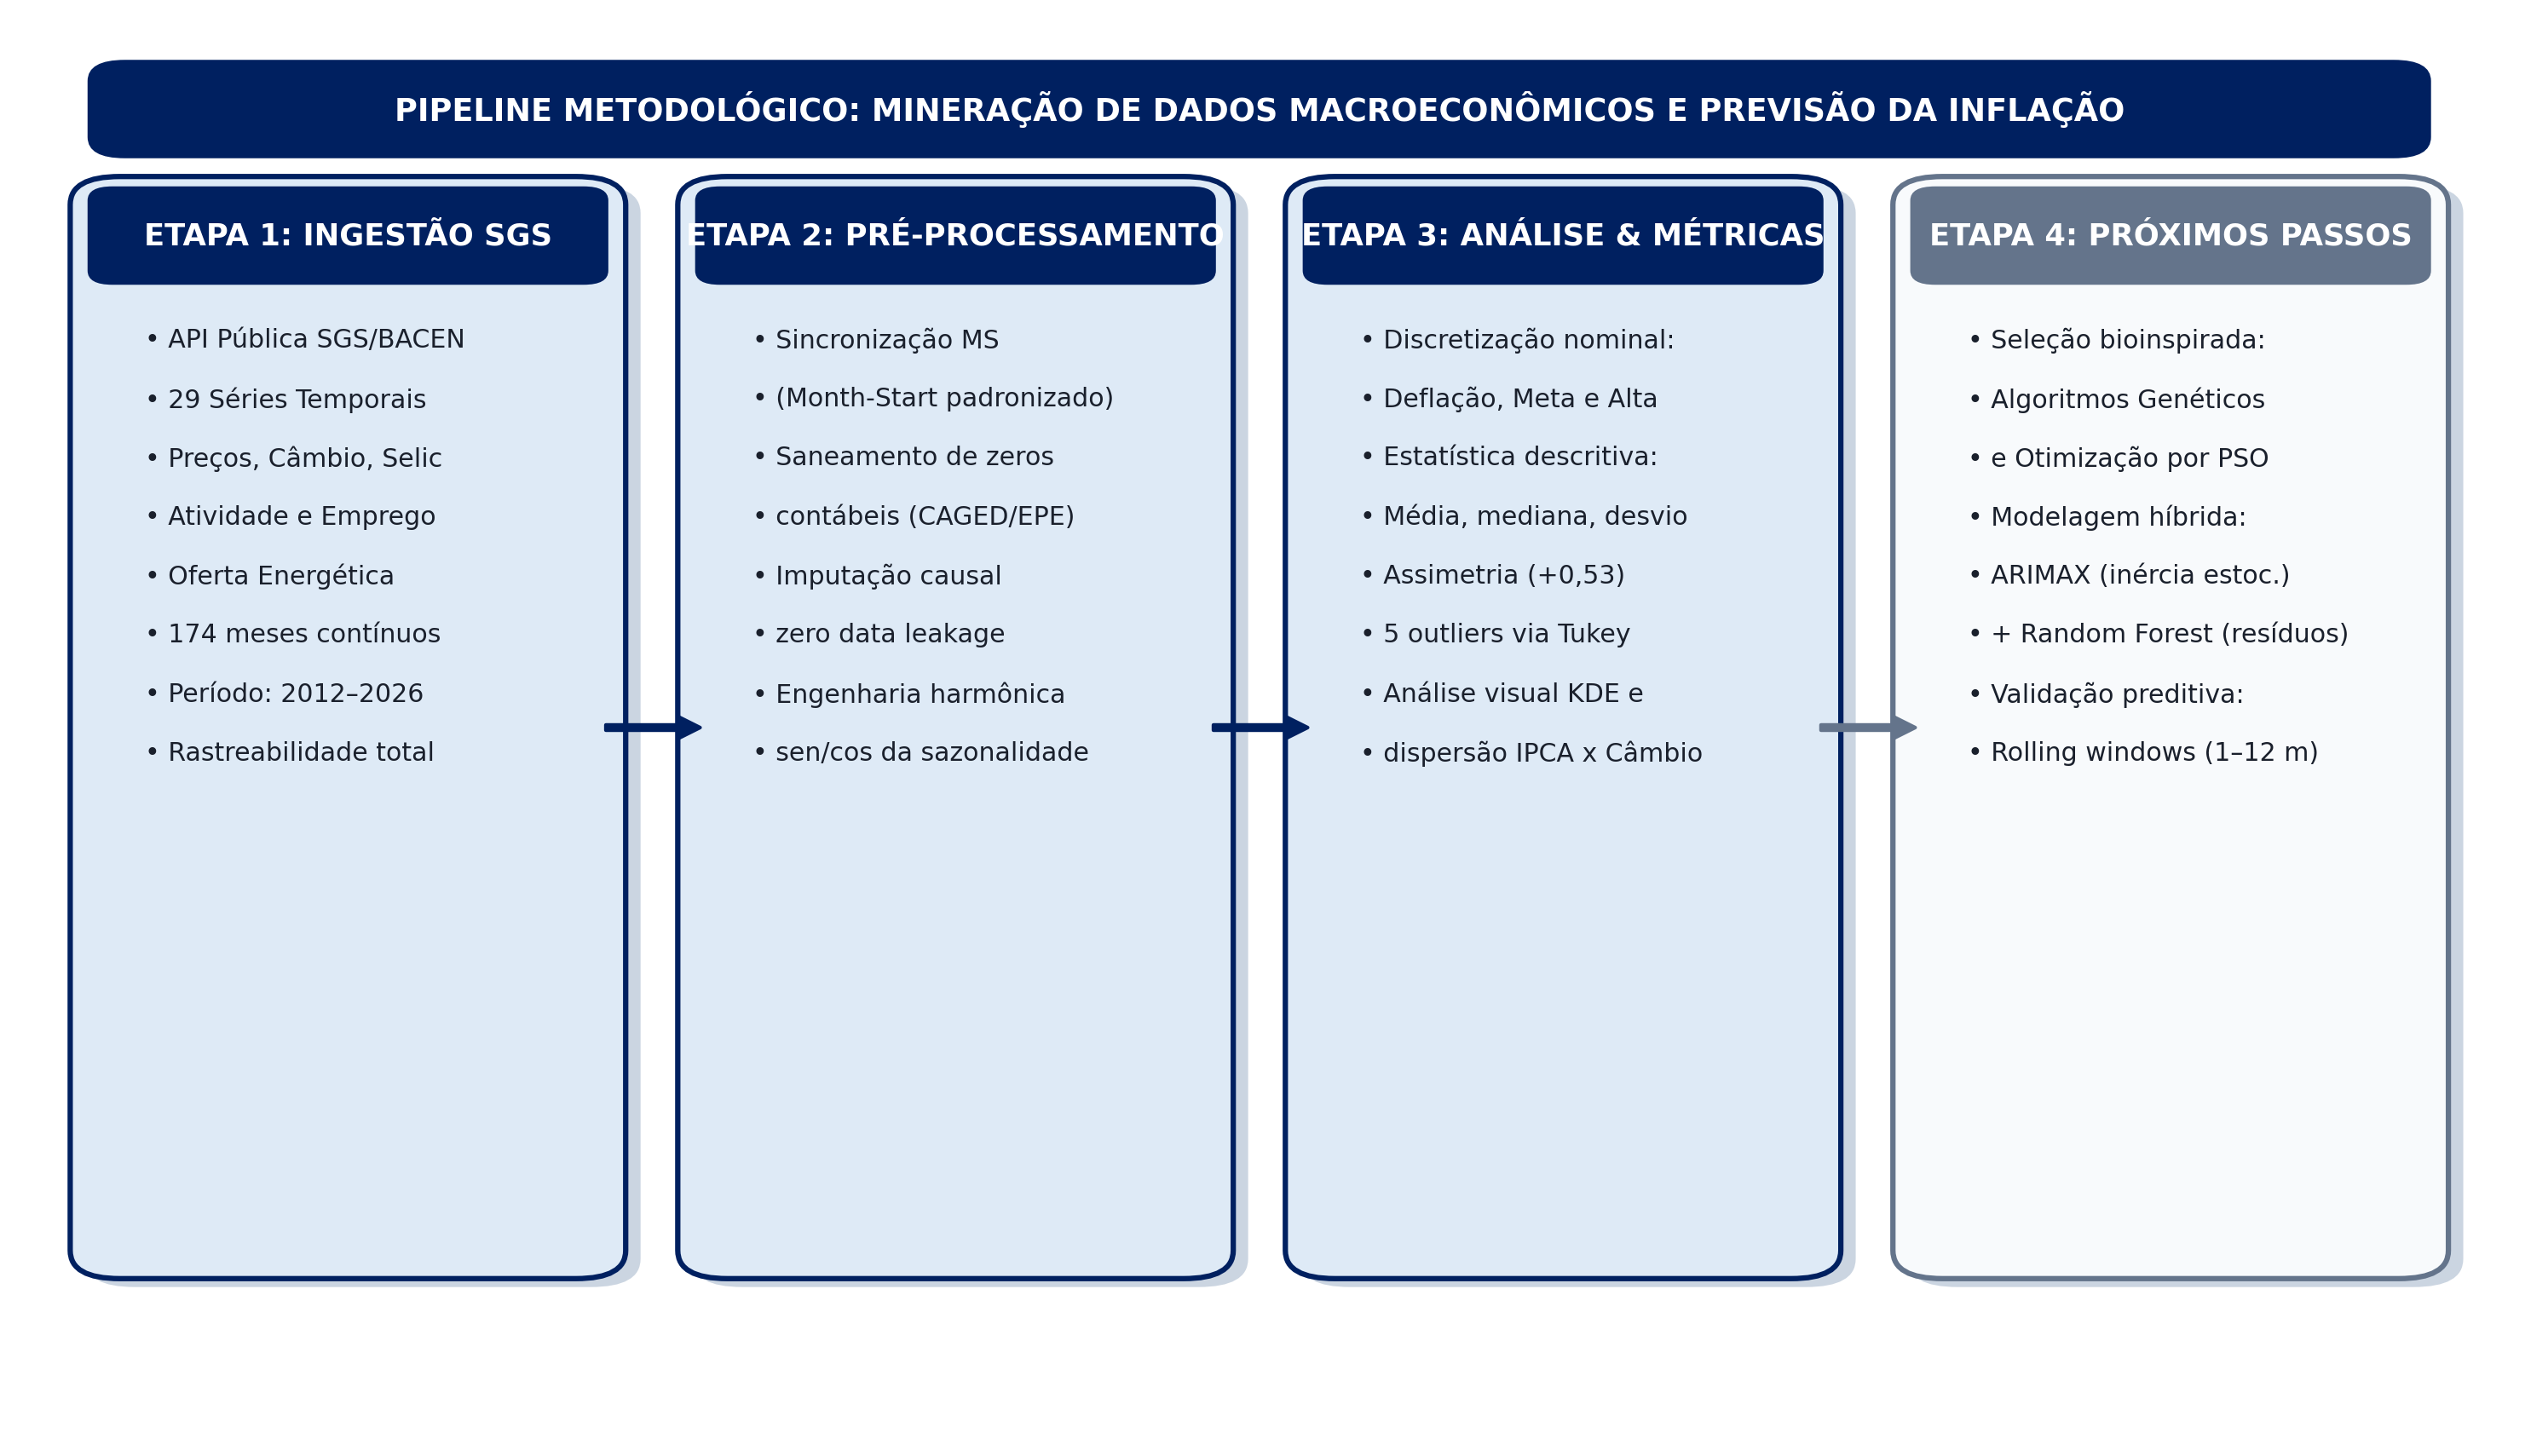
\includegraphics[width=0.92\textwidth]{Figura_0_Fluxograma_Metodologia.png}\[0.15cm]
    {\fontsize{8}{10}\selectfont \textbf{Fonte:} Autores (2026).}
\end{figure*}

\subsection{Stakeholders Envolvidos}
A concepção deste \textit{pipeline} integrou diretamente duas equipes especializadas com papéis complementares:
\begin{itemize}[leftmargin=1.5em]
    \item \textbf{Equipe de Engenharia da Computação / Mineração de Dados da POLI-UPE:} Responsável pelo desenho da arquitetura computacional, extração automatizada via APIs públicas, higienização, tratamento matemático de valores ausentes, análise descritiva e desenho algorítmico da futura seleção bioinspirada de atributos;
    \item \textbf{Especialistas de Domínio Econômico (Economistas):} Responsáveis pela validação conceitual das 29 variáveis macroeconômicas selecionadas, determinação dos canais de transmissão e defasagens da política monetária e parametrização dos regimes inflacionários nominais.
\end{itemize}

\subsection{Descrição da Base de Dados}
A base empírica foi extraída diretamente do Sistema Gerenciador de Séries Temporais (SGS) do Banco Central do Brasil \cite{ref2}, agregando fontes oficiais como IBGE, FGV, ANP, EPE e Ministério do Trabalho. O painel contempla 29 variáveis macroeconômicas distribuídas em seis dimensões analíticas: Preços ao Consumidor e Núcleos (IPCA Geral e 8 grupos setoriais do IBGE), Índices de Custos e Atacado (INPC, IGP-M, IGP-DI, IPC-BR), Câmbio e Finanças (PTAX, Selic, Reservas Internacionais), Nível de Atividade (PIB Mensal, Produção de Ovos), Mercado de Trabalho (Desemprego PNAD Contínua, Salário Mínimo, Estoques de Emprego CAGED) e Energia/Combustíveis (Refino de Petróleo, Consumo de Gasolina e Carga Elétrica Comercial, Residencial e Total).

\subsubsection{Delimitação Temporal e Justificativa Metodológica (2012 a 2026)}
A delimitação cronológica do estudo compreende o horizonte contínuo de janeiro de 2012 a junho de 2026, totalizando 174 observações mensais contínuas. A definição do marco inicial em 2012 é metodologicamente necessária para assegurar a homogeneidade dos dados, uma vez que o IBGE introduziu naquele ano duas reformas estruturais profundas: a revisão da estrutura de ponderação da cesta do IPCA com base nos microdados da Pesquisa de Orçamentos Familiares (POF 2008-2009) e a substituição definitiva da antiga Pesquisa Mensal de Emprego (PME) pela Pesquisa Nacional por Amostra de Domicílios Contínua (PNAD Contínua). 

A tentativa de retroagir a série temporal para períodos anteriores a 2012 introduziria quebras estruturais irreconciliáveis nos indicadores do mercado de trabalho e de desocupação, distorcendo os padrões estatísticos calculados pelos algoritmos de aprendizado. Por sua vez, a extensão do horizonte amostral até meados de 2026 garante a incorporação do ciclo econômico completo pós-pandemia, englobando as tensões inflacionárias decorrentes de gargalos nas cadeias produtivas globais, o choque energético internacional e as recentes flutuações das taxas de juros domésticas.

% --- INVERSÃO: 3.3 PRÉ-PROCESSAMENTO VEM ANTES DA DESCRITIVA ---
\subsection{Pré-processamento dos Dados}
\subsubsection{Procedimentos de Limpeza e Saneamento de Dados (Data Cleaning)}
As rotinas de pré-processamento resolveram três desafios práticos de engenharia de dados:
\begin{itemize}[leftmargin=1.5em]
    \item \textbf{Sincronização Cronológica:} Séries diárias (Selic e Câmbio PTAX) foram consolidadas em médias mensais de dias úteis com marcação temporal unificada no primeiro dia de cada competência (\textit{Month-Start} - MS);
    \item \textbf{Tratamento de Zeros Contábeis Estruturais:} Séries administrativas do CAGED e EPE apresentavam zeros resultantes de transições de sistemas cadastrais. Esses valores nulos artificiais foram convertidos em dados ausentes (\textit{missing data}) para não enviesar os cálculos de dispersão;
    \item \textbf{Imputação Causal sem Vazamento de Dados:} Lacunas pontuais de divulgação foram saneadas por interpolação linear estritamente retrospectiva (\textit{backward}), utilizando apenas observações passadas e garantindo ausência total de vazamento temporal (\textit{zero data leakage}).
\end{itemize}

\subsubsection{Técnicas de Redução de Dados e Engenharia de Atributos}
Para capturar a sazonalidade periódica anual sem inflacionar o espaço amostral com 11 variáveis binárias colineares (\textit{dummies}), implementou-se a codificação harmônica trigonométrica sobre o mês de competência  \in \{1, \dots, 12\}$:
\begin{equation}
\text{mes\_sin} = \sin\left(\frac{2\pi m}{12}\right), \quad \text{mes\_cos} = \cos\left(\frac{2\pi m}{12}\right)
\end{equation}
Essa formulação projeta o ciclo de 12 meses sobre o círculo unitário euclidiano, preservando a continuidade física e estocástica entre dezembro e janeiro.

\subsubsection{Dicionário de Dados da Base Consolidada Pré-Processada}
A base consolidada higienizada reúne 29 covariáveis e 174 meses contínuos. A Tabela 2 apresenta o dicionário técnico de dados estruturado.

\begin{table*}[t]
\centering
{\raggedright \fontsize{10}{12}\selectfont \textbf{\textcolor{REPABLUE}{Tabela 2 -}} Dicionário de Dados da Base Consolidada Pré-Processada (174 Meses, 2012–2026)\par}
\vspace{0.2cm}
\arrayrulecolor{REPABLUE}
\setlength{\arrayrulewidth}{1pt}
\renewcommand{\arraystretch}{1.15}
\fontsize{7.5}{9.5}\selectfont
\begin{tabularx}{\textwidth}{p{0.18\textwidth} p{0.14\textwidth} p{0.14\textwidth} p{0.24\textwidth} p{0.12\textwidth} X}
\hline
\textbf{Atributo} & \textbf{Código / Fonte} & \textbf{Tipo de Dado} & \textbf{Regra de Pré-processamento} & \textbf{Dimensão} & \textbf{Papel no Modelo Preditivo} \
\hline
\textbf{IPCA (Geral)} & SGS 433 (IBGE) & Float64 (\% a.m.) & Sem nulos; sincronização temporal contínua MS & Alvo Principal & Variável dependente contínua (alvo preditivo). \
\textbf{IPCA\_Alimentos} & SGS 1635 (IBGE) & Float64 (\% a.m.) & Sincronização MS; interpolação linear causal & Preços Setoriais & Covariável exógena - Choques climáticos e safra agrícola. \
\textbf{IPCA\_Habitacao} & SGS 1636 (IBGE) & Float64 (\% a.m.) & Alinhamento mensal; verificação de integridade & Preços Setoriais & Covariável exógena - Tarifas reguladas de energia e aluguéis. \
\textbf{IPCA\_Transportes} & SGS 1639 (IBGE) & Float64 (\% a.m.) & Sincronização MS; higienização & Preços Setoriais & Covariável exógena - Sensibilidade a combustíveis e tarifas. \
\textbf{USDBRL (Câmbio PTAX)} & SGS 3696 (BACEN) & Float64 (R$/US$) & Conversão diária para média mensal de dias úteis & Câmbio / Finanças & Covariável exógena - Mecanismo de \textit{pass-through} cambial. \
\textbf{SELIC} & SGS 4390 (BACEN) & Float64 (\% a.m.) & Conversão de taxa diária para média mensal útil & Câmbio / Finanças & Covariável exógena - Taxa básica de juros do COPOM. \
\textbf{Reservas\_Internac.} & SGS 3546 (BACEN) & Float64 (US$ Milhões) & Alinhamento mensal MS; saneamento de lacunas & Câmbio / Finanças & Covariável exógena - Liquidez externa e blindagem a choques. \
\textbf{IGP\_M} & SGS 189 (FGV) & Float64 (\% a.m.) & Sincronização MS; alinhamento de competência & Preços Setoriais & Covariável exógena - Indicador antecedente de custos no atacado. \
\textbf{PIB\_Mensal} & SGS 4380 (BACEN) & Float64 (R$ Milhões) & Tratamento de atrasos de divulgação; MS & Atividade Econômica & Covariável exógena - Proxy de nível de atividade agregada. \
\textbf{Desemprego (PNAD)} & SGS 24369 (IBGE) & Float64 (\% da PEA) & Truncamento pós-2012; interpolação causal & Mercado de Trabalho & Covariável exógena - Dinâmica da desocupação (Curva de Phillips). \
\textbf{Estoque\_Empregos\_Total} & SGS 28763 (CAGED) & Float64 (Mil vínculos) & Zeros tratados como ausentes; interpolação causal & Mercado de Trabalho & Covariável exógena - Saldo mensal de emprego formal. \
\textbf{Consumo\_Gasolina} & SGS 1393 (ANP) & Float64 (m³) & Sincronização MS; zeros tratados como ausentes & Energia / Combustíveis & Covariável exógena - Consumo automotivo e transporte. \
\textbf{Consumo\_Energia\_Total} & SGS 1406 (EPE) & Float64 (MWh) & Sincronização mensal MS; verificação causal & Energia / Combustíveis & Covariável exógena - Demanda física global de eletricidade. \
\textbf{Regime de Inflação} & IBGE / CMN & Categórico Nominal & Discretização paramétrica: Deflação, Meta e Alta & Governança / CMN & Atributo nominal derivado qualitativo. \
\textbf{mes\_sin / mes\_cos} & Engenharia Temporal & Float64 (Adimensional) & Harmônicas trigonométricas anuais $\sin$ e $\cos$ & Sazonalidade & Covariáveis cíclicas periódicas contínuas. \
\hline
\end{tabularx}
\vspace{0.1cm}
{\raggedright \fontsize{8}{10}\selectfont \textbf{Fonte:} Elaboração própria com base no pipeline computacional desenvolvido e validado com os especialistas de domínio (2026).\par}
\end{table*}

\subsection{Análise Exploratória e Descritiva dos Dados}
\subsubsection{Distribuição de Frequências e Métricas Descritivas}
Para o atributo numérico contínuo principal ( = \text{IPCA}$), a análise descritiva da série de 174 meses aponta:
\begin{itemize}[leftmargin=1.5em]
    \item Média mensal: 0,447\% a.m.;
    \item Mediana: 0,380\% a.m.;
    \item Desvio padrão: 0,344\%;
    \item Mínimo: -0,680\% a.m. (julho/2022, deflação por desoneração de combustíveis);
    \item Máximo: 1,950\% a.m. (março/2015, realinhamento de tarifas represadas);
    \item Coeficiente de Assimetria: +0,53 (assimetria positiva à direita);
    \item Curtose: 3,82 (distribuição leptocúrtica com caudas pesadas).
\end{itemize}

O atributo nominal derivado (\textbf{Regime de Inflação}) foi discretizado com base nas metas do BACEN em: Deflação (IPCA $\le$ 0\%), Meta (0\% $<$ IPCA $\le$ 0,55\%) e Alta (IPCA $>$ 0,55\% a.m.). A Tabela 3 apresenta a distribuição percentual amostral.

\begin{table}[htbp]
\centering
{\raggedright \fontsize{10}{12}\selectfont \textbf{\textcolor{REPABLUE}{Tabela 3 -}} Distribuição de Frequência do Atributo Nominal (Regime de Inflação)\par}
\vspace{0.2cm}
\arrayrulecolor{REPABLUE}
\setlength{\arrayrulewidth}{1pt}
\renewcommand{\arraystretch}{1.15}
\fontsize{8}{10}\selectfont
\begin{tabularx}{\columnwidth}{p{0.22\columnwidth} p{0.32\columnwidth} >{\centering\arraybackslash}p{0.20\columnwidth} >{\centering\arraybackslash}p{0.18\columnwidth}}
\hline
\textbf{Regime Nominal} & \textbf{Critério Paramétrico} & \textbf{Frequência Absoluta} & \textbf{Frequência Relativa (\%)} \
\hline
\textbf{Deflação} & $\text{IPCA} \le 0,00\%$ & 27 & 15,52\% \
\textbf{Meta} & zsh,00\% < \text{IPCA} \le 0,55\%$ & 77 & 44,25\% \
\textbf{Alta} & $\text{IPCA} > 0,55\%$ & 70 & 40,23\% \
\hline
\textbf{Total} & \textbf{Amostra Global (2012–2026)} & \textbf{174} & \textbf{100,00\%} \
\hline
\end{tabularx}
\vspace{0.1cm}
{\raggedright \fontsize{8}{10}\selectfont \textbf{Fonte:} Elaboração própria a partir dos microdados do SGS/BACEN e metas do CMN (2026).\par}
\end{table}

\subsubsection{Análise Visual dos Dados: Histograma, Boxplot e Dispersão}
A Figura 2 confirma a concentração da inflação entre 0,10\% e 0,60\% ao mês. A proximidade entre média e mediana reforça a regularidade central, enquanto a assimetria positiva (+0,53) demonstra que choques inflacionários são significativamente mais severos do que quedas de preço.

\begin{figure}[htbp]
    \centering
    {\fontsize{10}{12}\selectfont \textbf{Figura 2} – Histograma e Densidade Empírica (KDE) do IPCA (2012–2026)}\[0.2cm]
    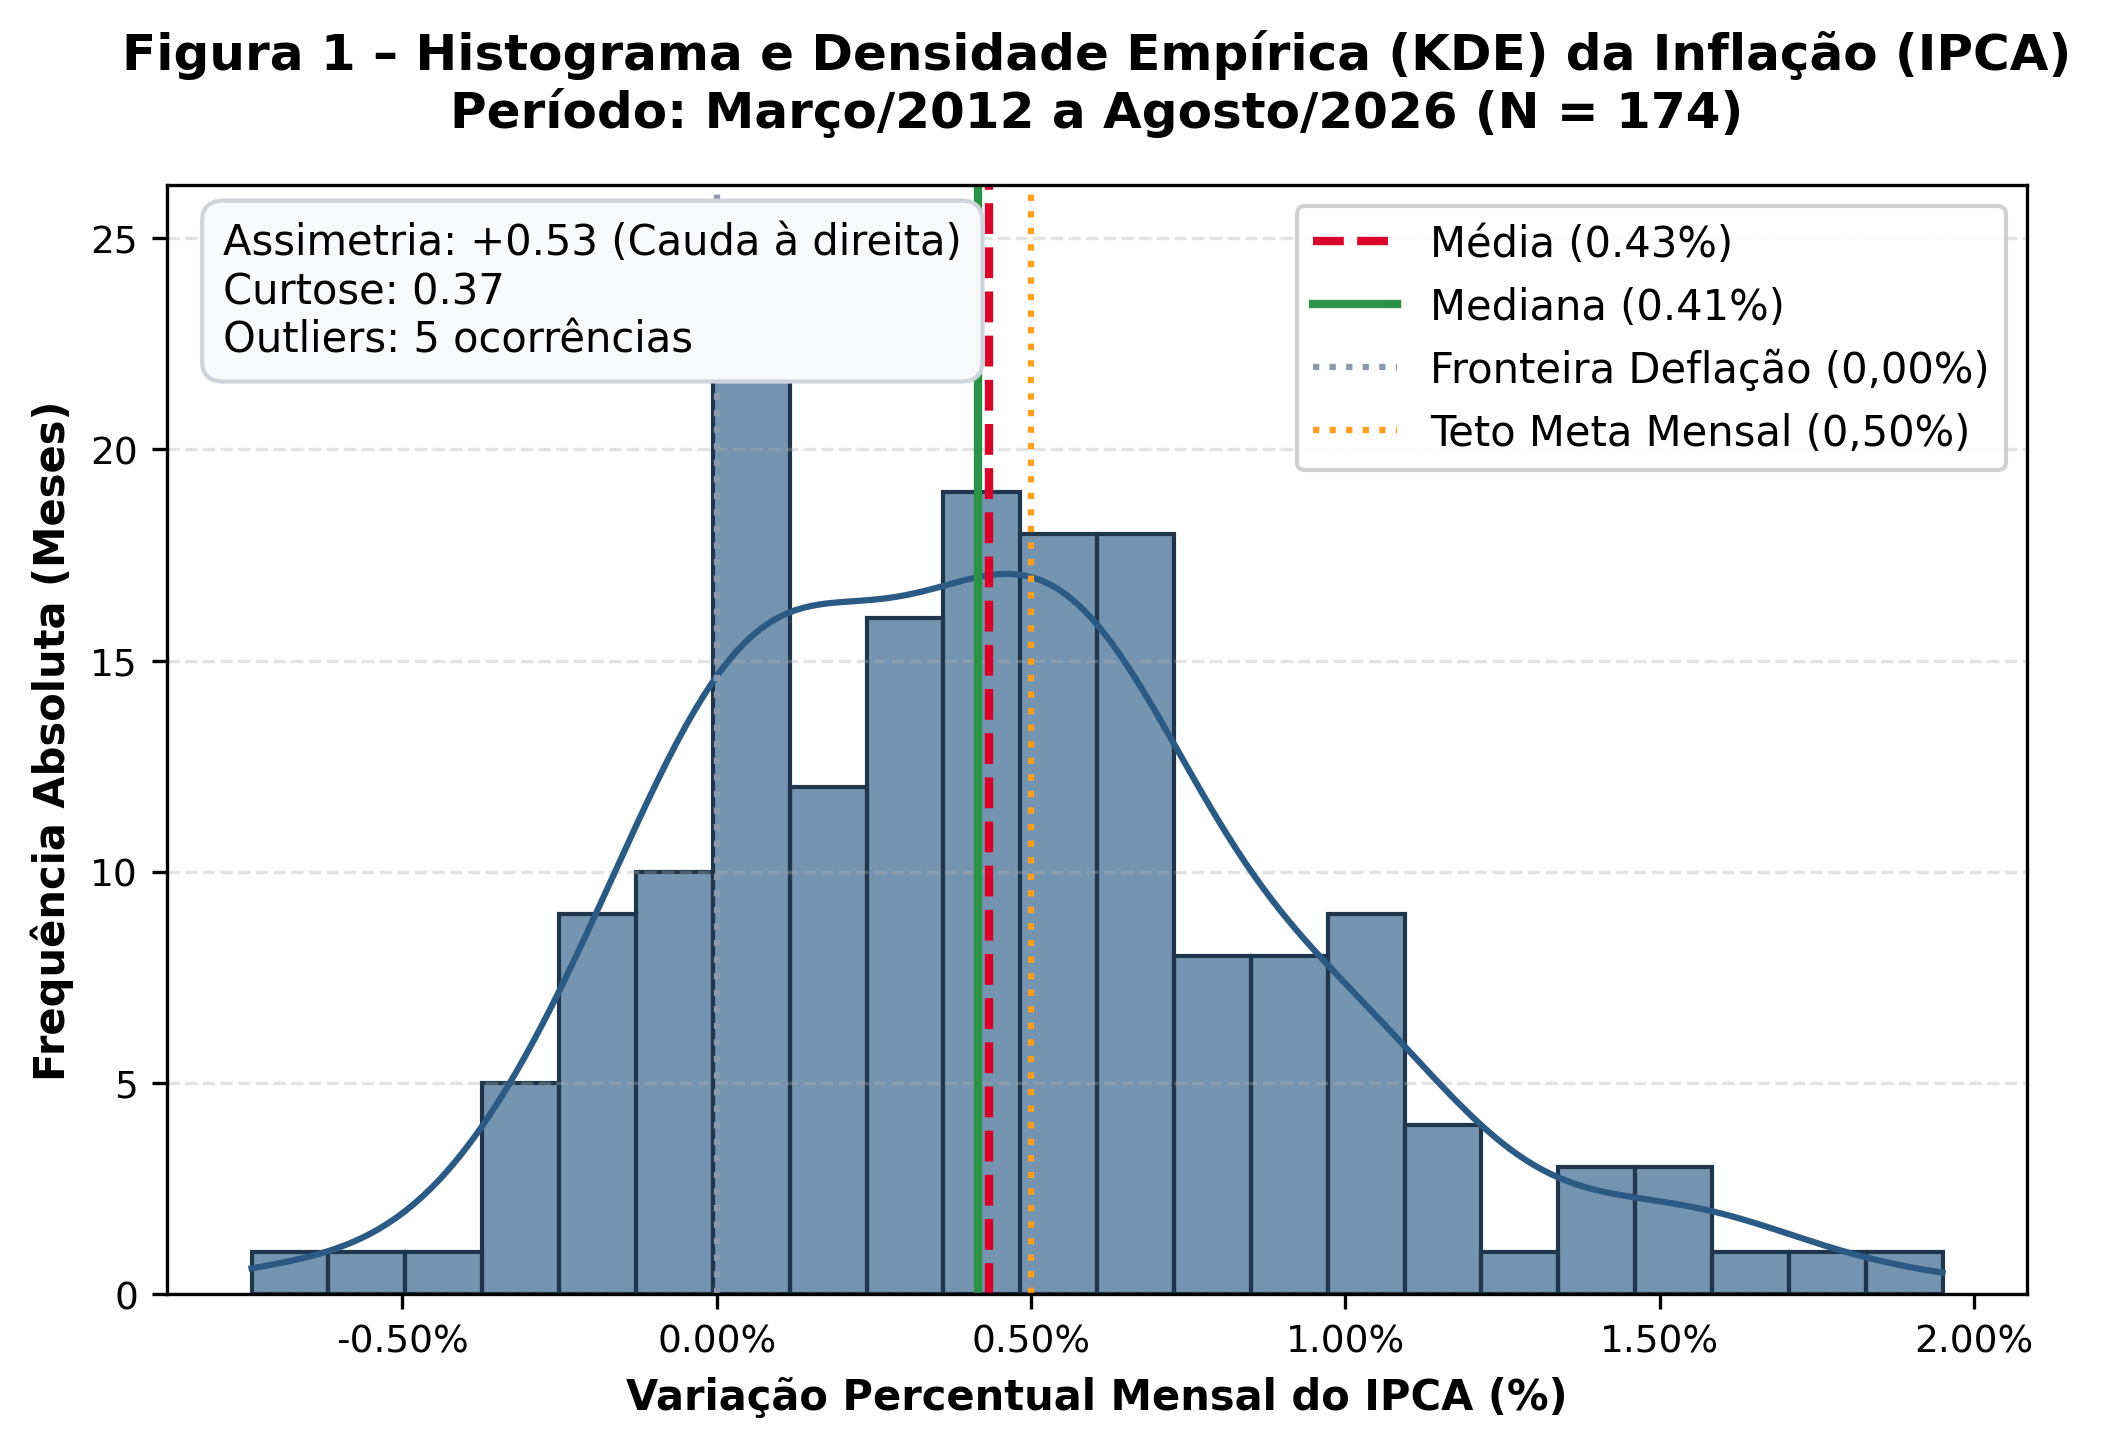
\includegraphics[width=\columnwidth]{Figura_1_Histograma_IPCA.png}\[0.15cm]
    {\fontsize{8}{10}\selectfont \textbf{Fonte:} Autores (2026).}
\end{figure}

O Diagrama de Caixa (\textit{Boxplot}) univariado na Figura 3 identifica 5 \textit{outliers} severos pelo critério de Tukey (IQR): março/2015 (+1,95\%), outubro/2020 (+1,72\%), novembro/2020 (+1,61\%), dezembro/2020 (+1,58\%) e dezembro/2021 (+1,58\%), decorrentes de choques em carnes e restrições de cadeias de suprimentos globais. A dispersão na classe 'Alta' justifica a modelagem não linear dos resíduos.

\begin{figure}[htbp]
    \centering
    {\fontsize{10}{12}\selectfont \textbf{Figura 3} – Diagrama de Caixa (\textit{Boxplot}) do IPCA Global e por Regimes}\[0.2cm]
    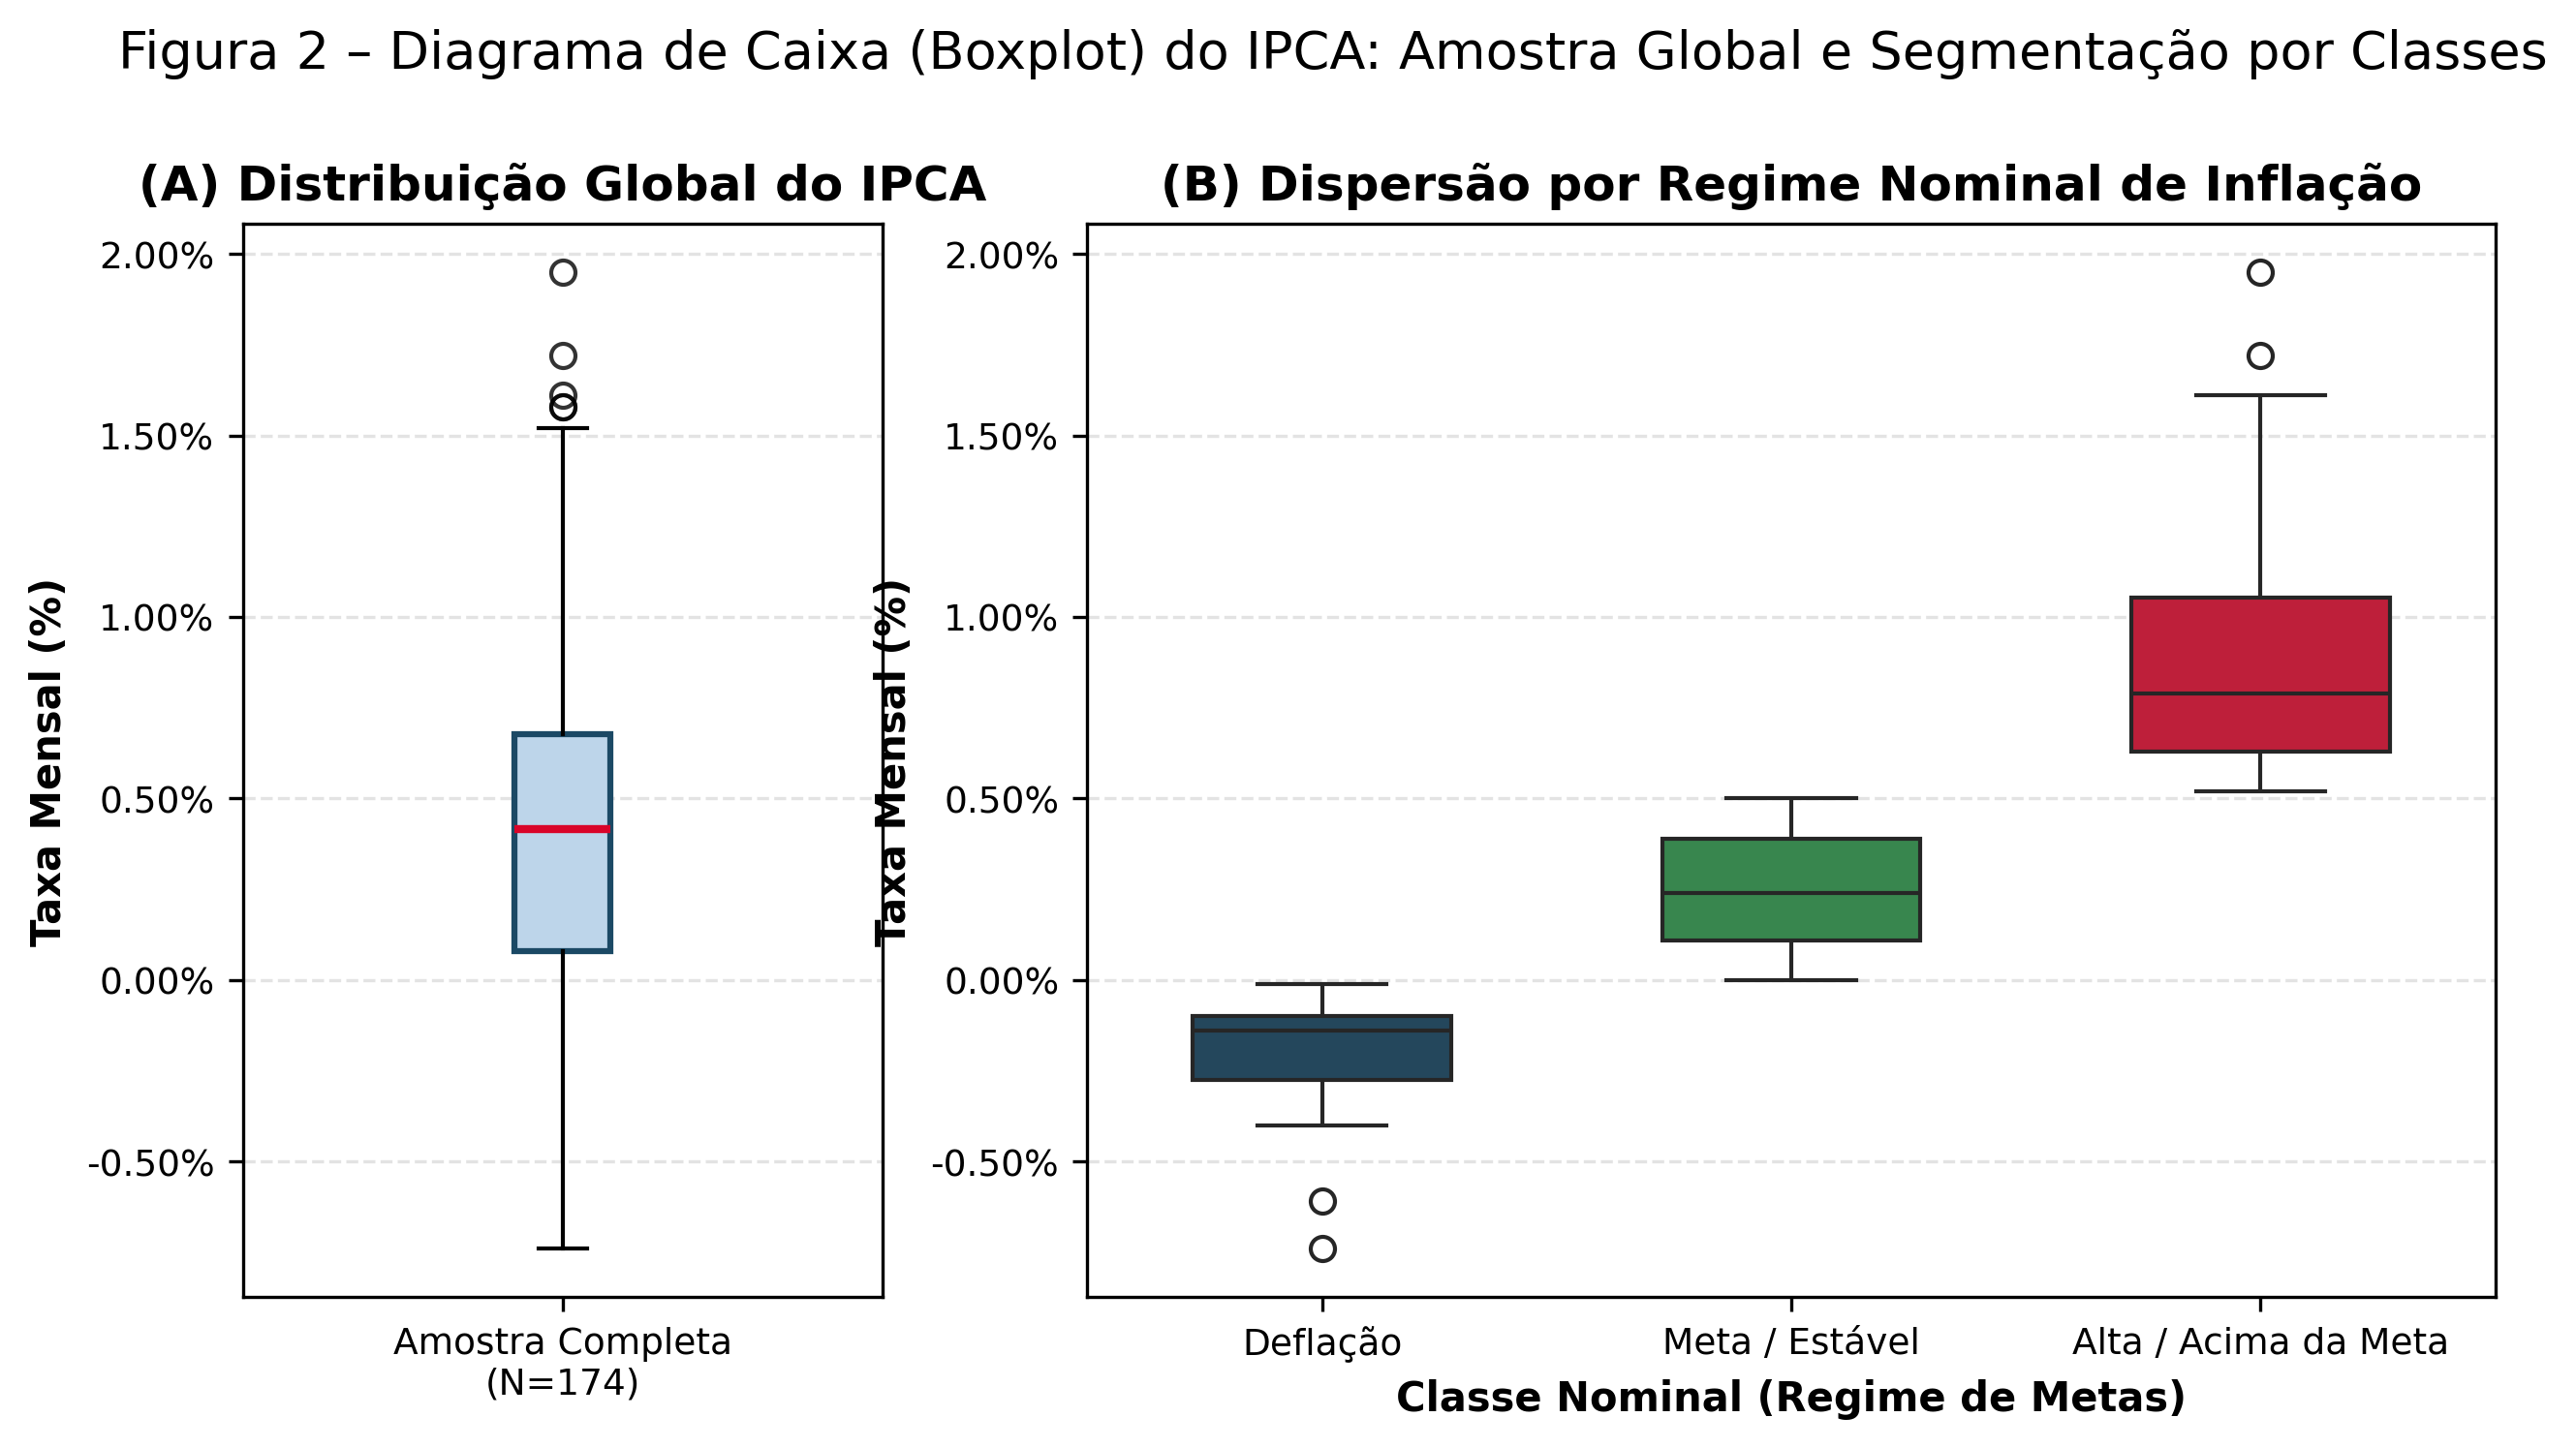
\includegraphics[width=\columnwidth]{Figura_2_Boxplot_IPCA.png}\[0.15cm]
    {\fontsize{8}{10}\selectfont \textbf{Fonte:} Autores (2026).}
\end{figure}

O gráfico de dispersão da Figura 4 evidencia a relação positiva entre desvalorização cambial e inflação (\textit{pass-through} cambial). À medida que a cotação do dólar opera em patamares elevados, a incidência de meses no regime de 'Alta' aumenta perceptivelmente.

\begin{figure}[htbp]
    \centering
    {\fontsize{10}{12}\selectfont \textbf{Figura 4} – Gráfico de Dispersão entre IPCA e Câmbio (USDBRL) por Regime}\[0.2cm]
    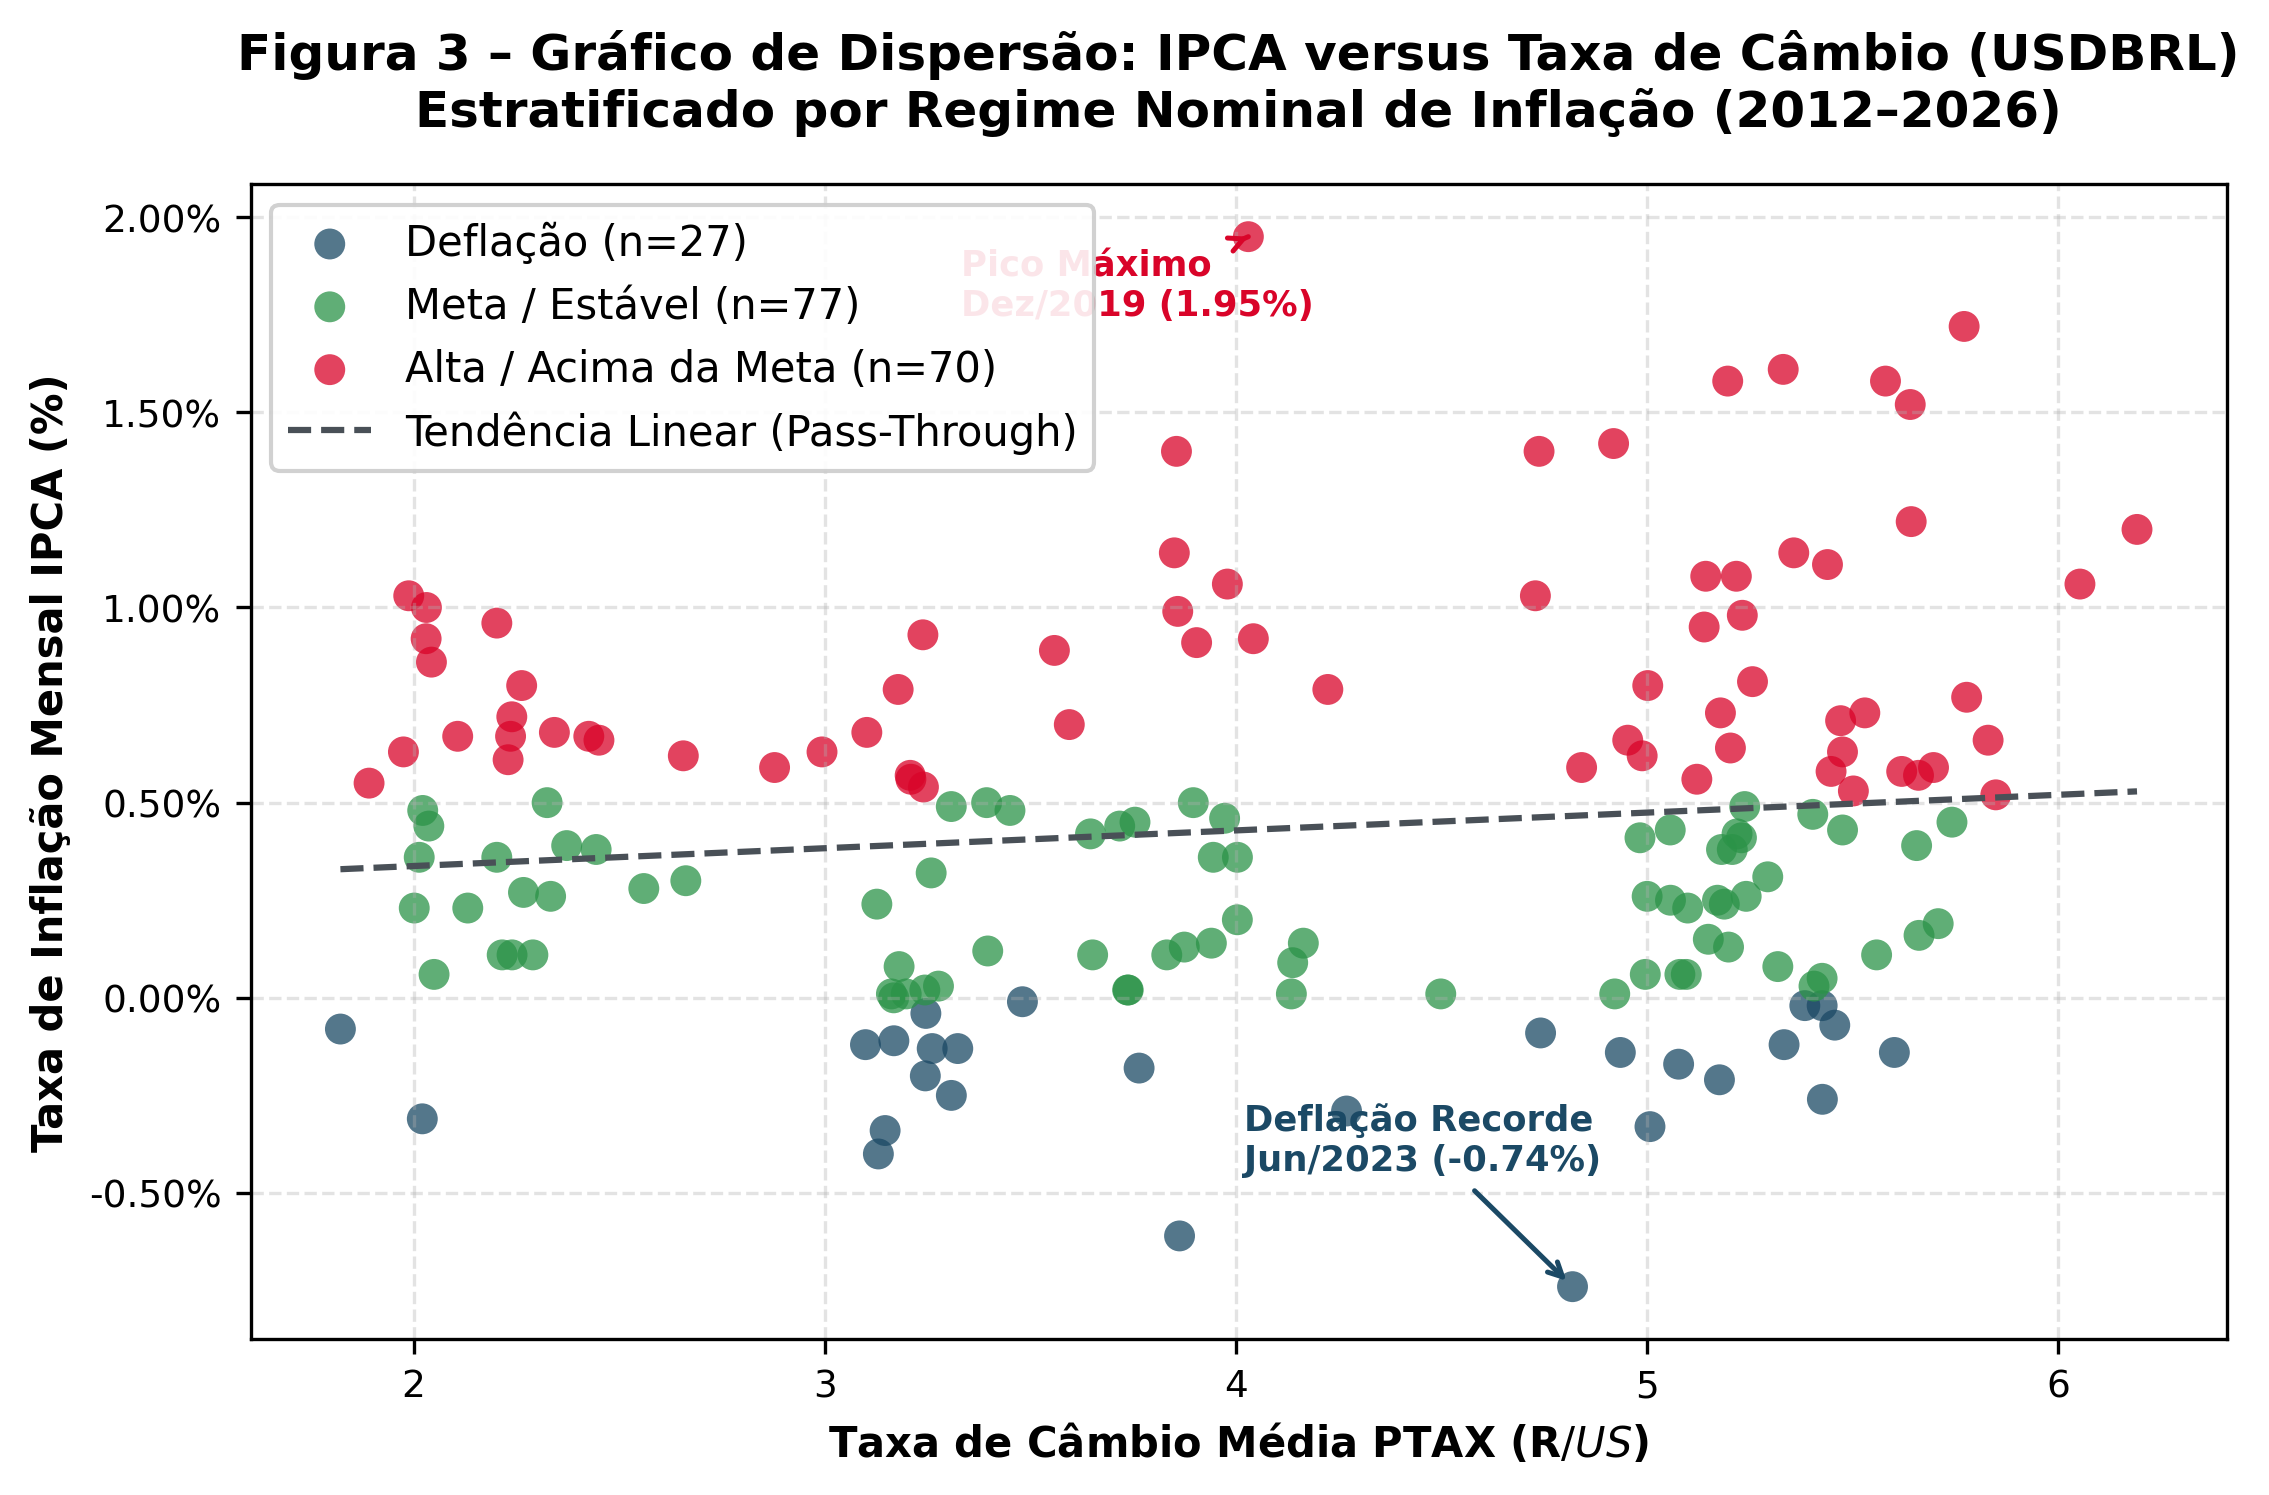
\includegraphics[width=\columnwidth]{Figura_3_Dispersao_IPCA_Cambio.png}\[0.15cm]
    {\fontsize{8}{10}\selectfont \textbf{Fonte:} Autores (2026).}
\end{figure}

A Figura 5 sintetiza a distribuição amostral: 44,25\% dos meses situaram-se na meta, 40,23\% em patamares elevados e 15,52\% em deflação (provocada por desonerações tributárias temporárias e contrações severas de demanda).

\begin{figure}[htbp]
    \centering
    {\fontsize{10}{12}\selectfont \textbf{Figura 5} – Proporção Percentual dos Regimes Nominais de Inflação (N = 174)}\[0.2cm]
    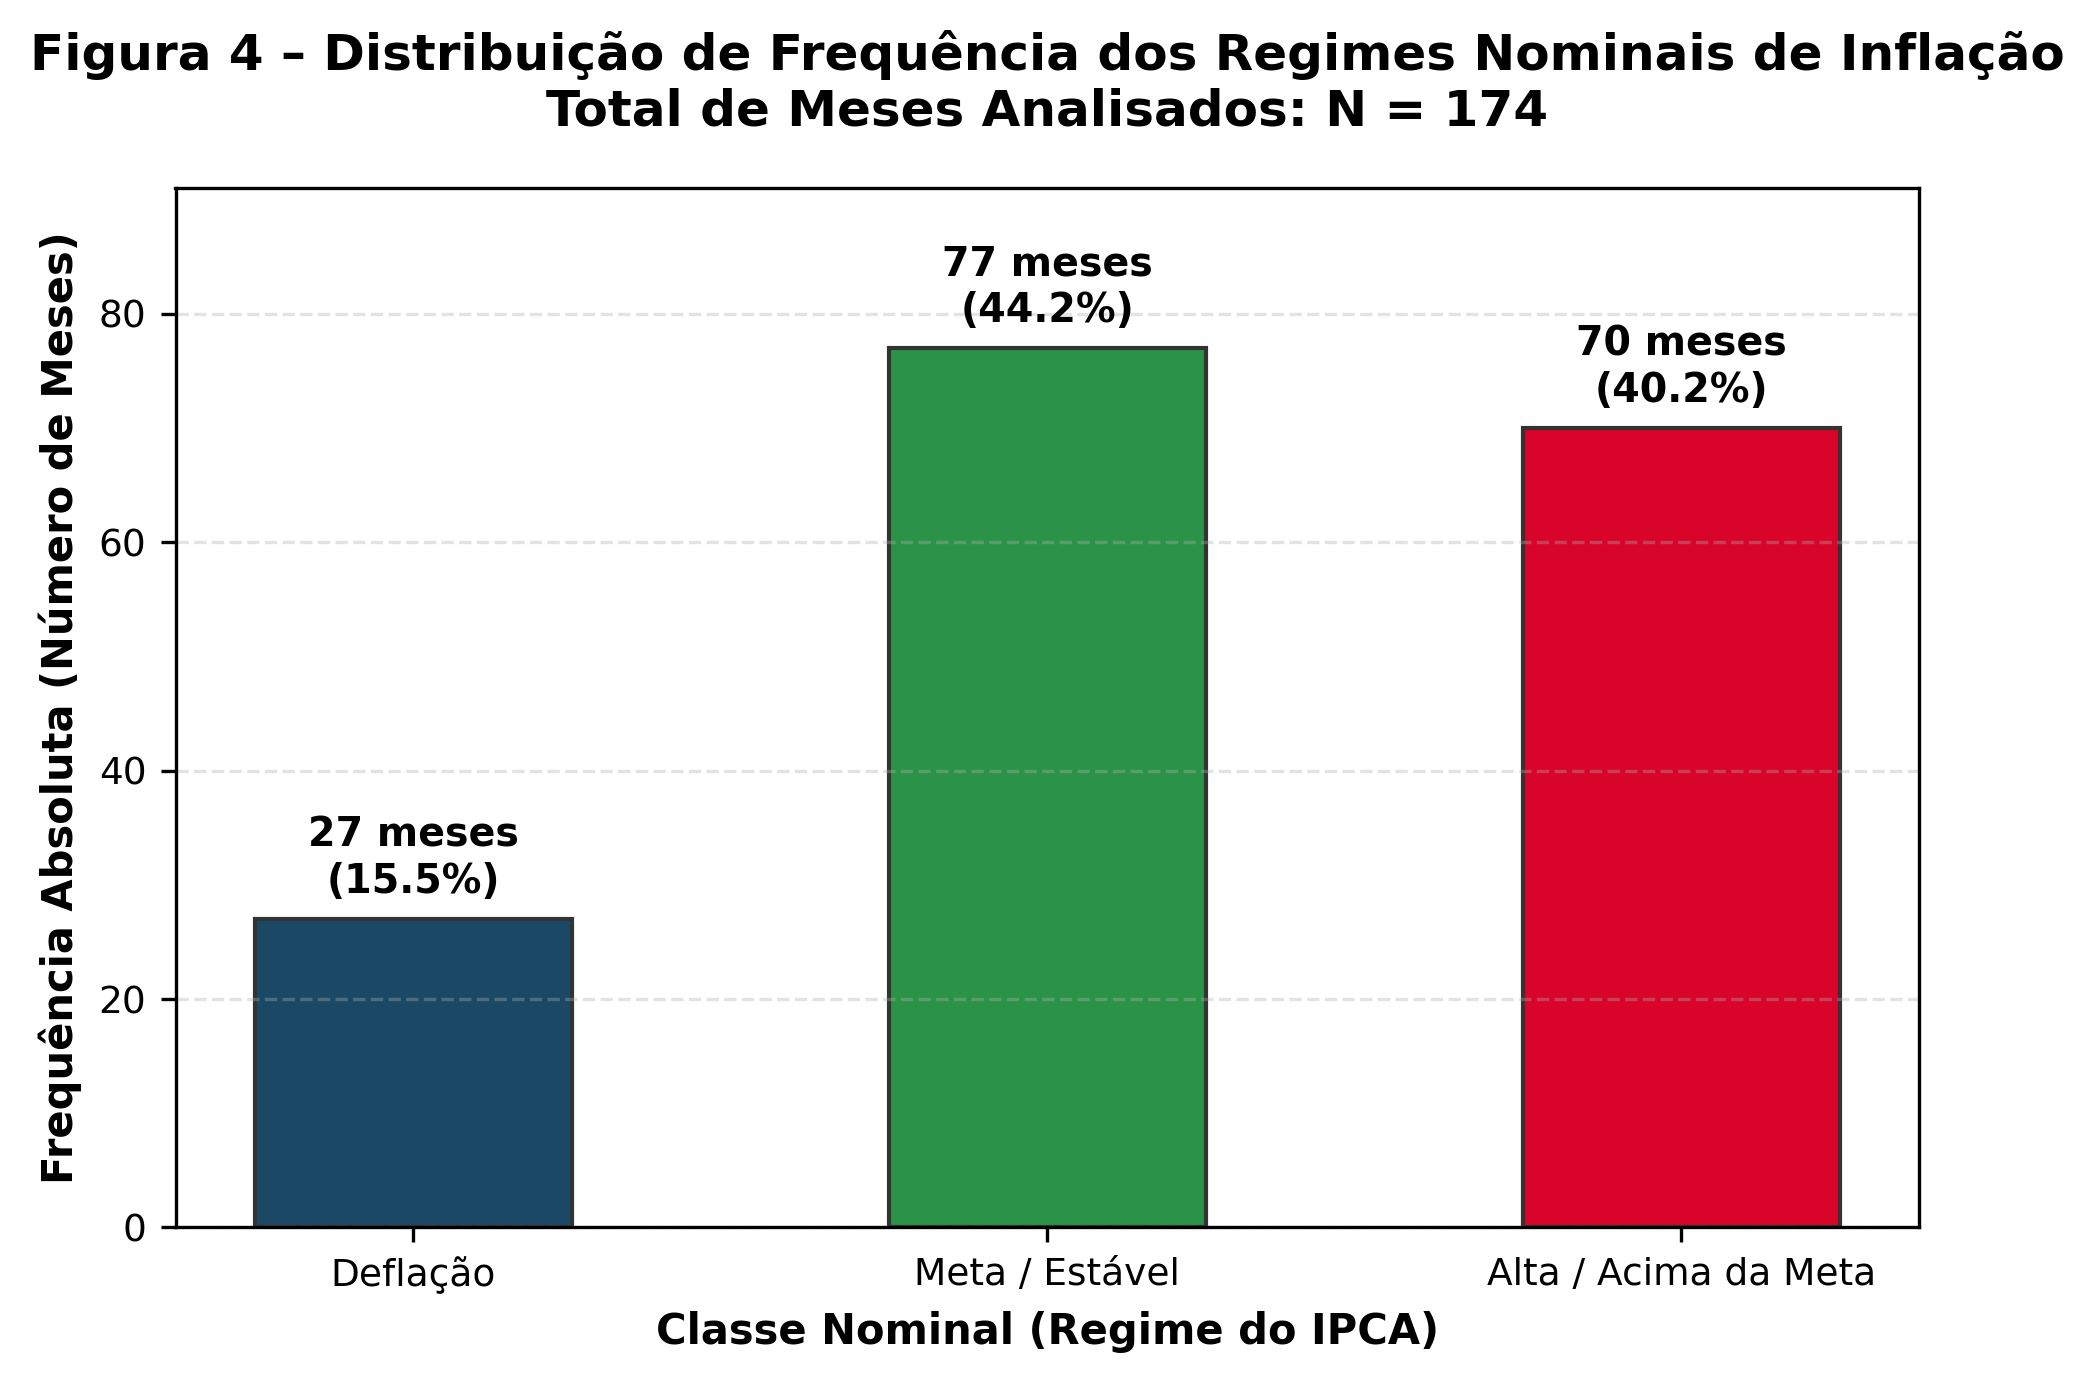
\includegraphics[width=\columnwidth]{Figura_4_Distribuicao_Regimes.png}\[0.15cm]
    {\fontsize{8}{10}\selectfont \textbf{Fonte:} Autores (2026).}
\end{figure}

\subsubsection{Governança, Integridade e Requisitos de Qualidade}
As rotinas de ingestão via API SGS/BACEN contam com validação de tipos, verificação de limites estocásticos e rastreabilidade completa de código, assegurando a reprodutibilidade dos experimentos computacionais.

% =====================================================================
\subsection{Metodologia Experimental de Agrupamento: Sazonalidade e Regimes de Ouro e Juros}
A identificação de padrões não supervisionados na economia brasileira requer rigor na especificação do espaço de atributos. Fenômenos sazonais e ciclos macroeconômicos operam em naturezas temporais distintas:
\begin{itemize}
    \item \textbf{Sazonalidade:} Processo determinístico e recorrente de frequência intra-anual fixa ($S = 12$ meses);
    \item \textbf{Ciclos Macroeconômicos (Ouro e Juros):} Processos estocásticos plurianuais governados por decisões de política monetária e choques geopolíticos internacionais (ciclos de 24 a 60 meses).
\end{itemize}

A unificação ingênua de atributos calendáricos com variáveis financeiras num único espaço euclidiano distorce o cálculo métrico e resulta em agrupamentos espúrios (\textit{spurious clustering}). Para superar essa limitação, este projeto adotou o framework desacoplado em duas camadas (\textit{Two-Tier Decoupled Clustering Framework}), complementado por uma análise de interação cruzada:

\subsubsection{Protocolo Experimental da Camada 1 (Sazonalidade Intra-Anual)}
Selecionaram-se os 7 componentes desagregados de preços do IPCA apurados pelo IBGE (\texttt{Transportes}, \texttt{Alimentação e Bebidas}, \texttt{Habitação}, \texttt{Saúde}, \texttt{Vestuário}, \texttt{Educação} e \texttt{Despesas Pessoais}). Aplicou-se o escalonamento $Z$-Score em cada componente $j$ ($z_{i,j} = \frac{x_{i,j} - \mu_j}{\sigma_j}$), submetendo a matriz ao agrupamento hierárquico com critério de Ward.

\subsubsection{Protocolo Experimental da Camada 2 (Regimes de Inflação, Ouro e Juros)}
Construiu-se um vetor tridimensional estacionário para cada mês $t$ ($N = 173$ meses): (i) $\text{IPCA}_t$ (\% a.m.); (ii) $\Delta \text{SELIC}_t = \text{SELIC}_t - \text{SELIC}_{t-1}$ (aceleração monetária em p.p.); e (iii) $\Delta \% \text{Ouro}_{BRL,t}$ (retorno percentual mensal do ouro físico internacional GLD convertido para Reais via PTAX), capturando risco global e câmbio \cite{ref21, ref22}. O juro real \textit{ex-post} ($r_t = \text{SELIC}_t - \text{IPCA}_t$) foi preservado como variável de auditoria.

\subsubsection{Métricas de Validação Interna e Avaliação Estatística}
A determinação de $k \in \{2, 3, 4, 5, 6\}$ baseou-se no Coeficiente de Silhueta (\textit{Silhouette Score} -- $s_i$), Índice de Davies-Bouldin ($DB$) e Índice de Calinski-Harabasz ($CH$). Na Camada 3, a hipótese de independência estocástica entre sazonalidade e regimes foi submetida ao Teste Qui-Quadrado de Pearson ($\chi^2$).

\section{RESULTADOS OBTIDOS E DISCUSSÕES}
% =====================================================================

\subsection{Resultados Obtidos na Clusterização de Sazonalidade e Regimes Macroeconômicos}
A aplicação experimental do \textit{Two-Tier Decoupled Framework} forneceu evidências empíricas contundentes sobre a arquitetura da inflação brasileira.

\subsubsection{Camada 1: Sazonalidade e Choques Estruturais dos Componentes do IPCA}
A Tabela \ref{tab:metricas_camada1} sintetiza as métricas de validação interna do agrupamento hierárquico de Ward aplicado aos 7 componentes desagregados do IPCA ($N = 174$ meses).

\begin{table}[H]
\centering
\caption{Métricas de Validação Interna do Agrupamento Hierárquico (Ward) -- Camada 1}
\label{tab:metricas_camada1}
\small
\begin{tabular}{cccc}
\toprule
\textbf{Clusters ($k$)} & \textbf{Silhouette} & \textbf{Davies-Bouldin ($DB$)} & \textbf{Calinski-Harabasz ($CH$)} \\
\midrule
$k = 2$ & 0,324 & 1,085 & 63,8 \\
$k = 3$ & 0,132 & 1,837 & 44,5 \\
\textbf{$k = 4$ (Adotado)} & \textbf{0,155} & \textbf{1,796} & \textbf{38,6} \\
$k = 5$ & 0,175 & 1,631 & 34,2 \\
$k = 6$ & 0,179 & 1,587 & 31,9 \\
\bottomrule
\end{tabular}
\end{table}

A solução com $k=4$ foi adotada por isolar com precisão cirúrgica os quatro regimes calendáricos. A Figura \ref{fig:dendro_sazonal} ilustra o dendrograma resultante, com linha tracejada vermelha no corte ótimo em altura 14,0.

\begin{figure}[H]
\centering
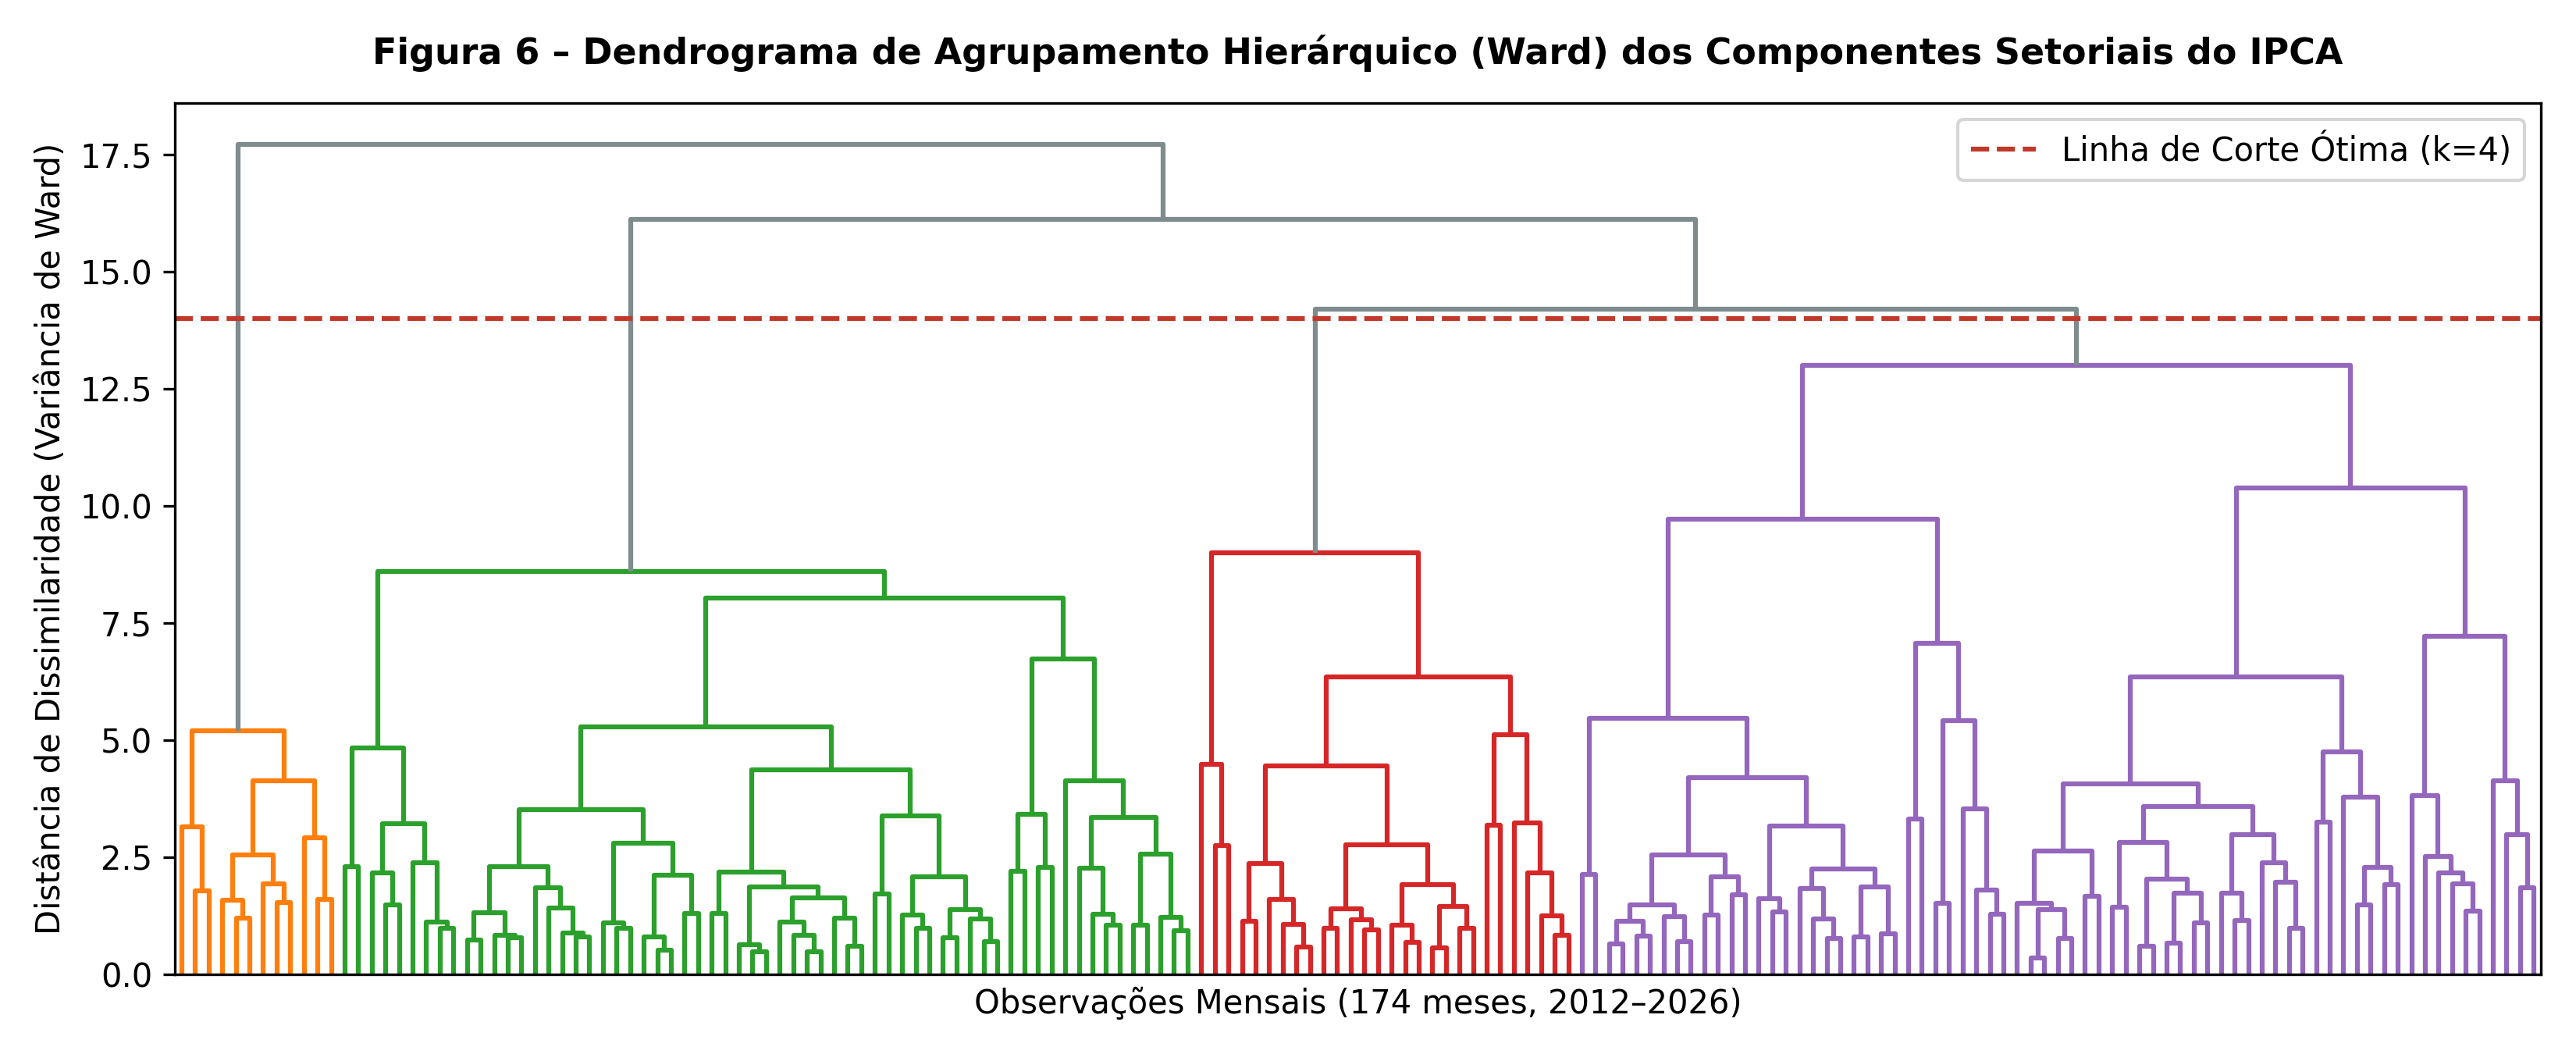
\includegraphics[width=0.92\linewidth]{Figura_6_Dendrograma_Sazonalidade_IPCA.png}
\caption{Dendrograma de Agrupamento Hierárquico (critério de Ward) dos Componentes Setoriais do IPCA (2012--2026). Linha tracejada indica corte em $k=4$.}
\label{fig:dendro_sazonal}
\end{figure}

O heatmap da Figura \ref{fig:heat_sazonal} detalha os desvios-padrão médios de cada componente setorial nos quatro grupos sazonais.

\begin{figure}[H]
\centering
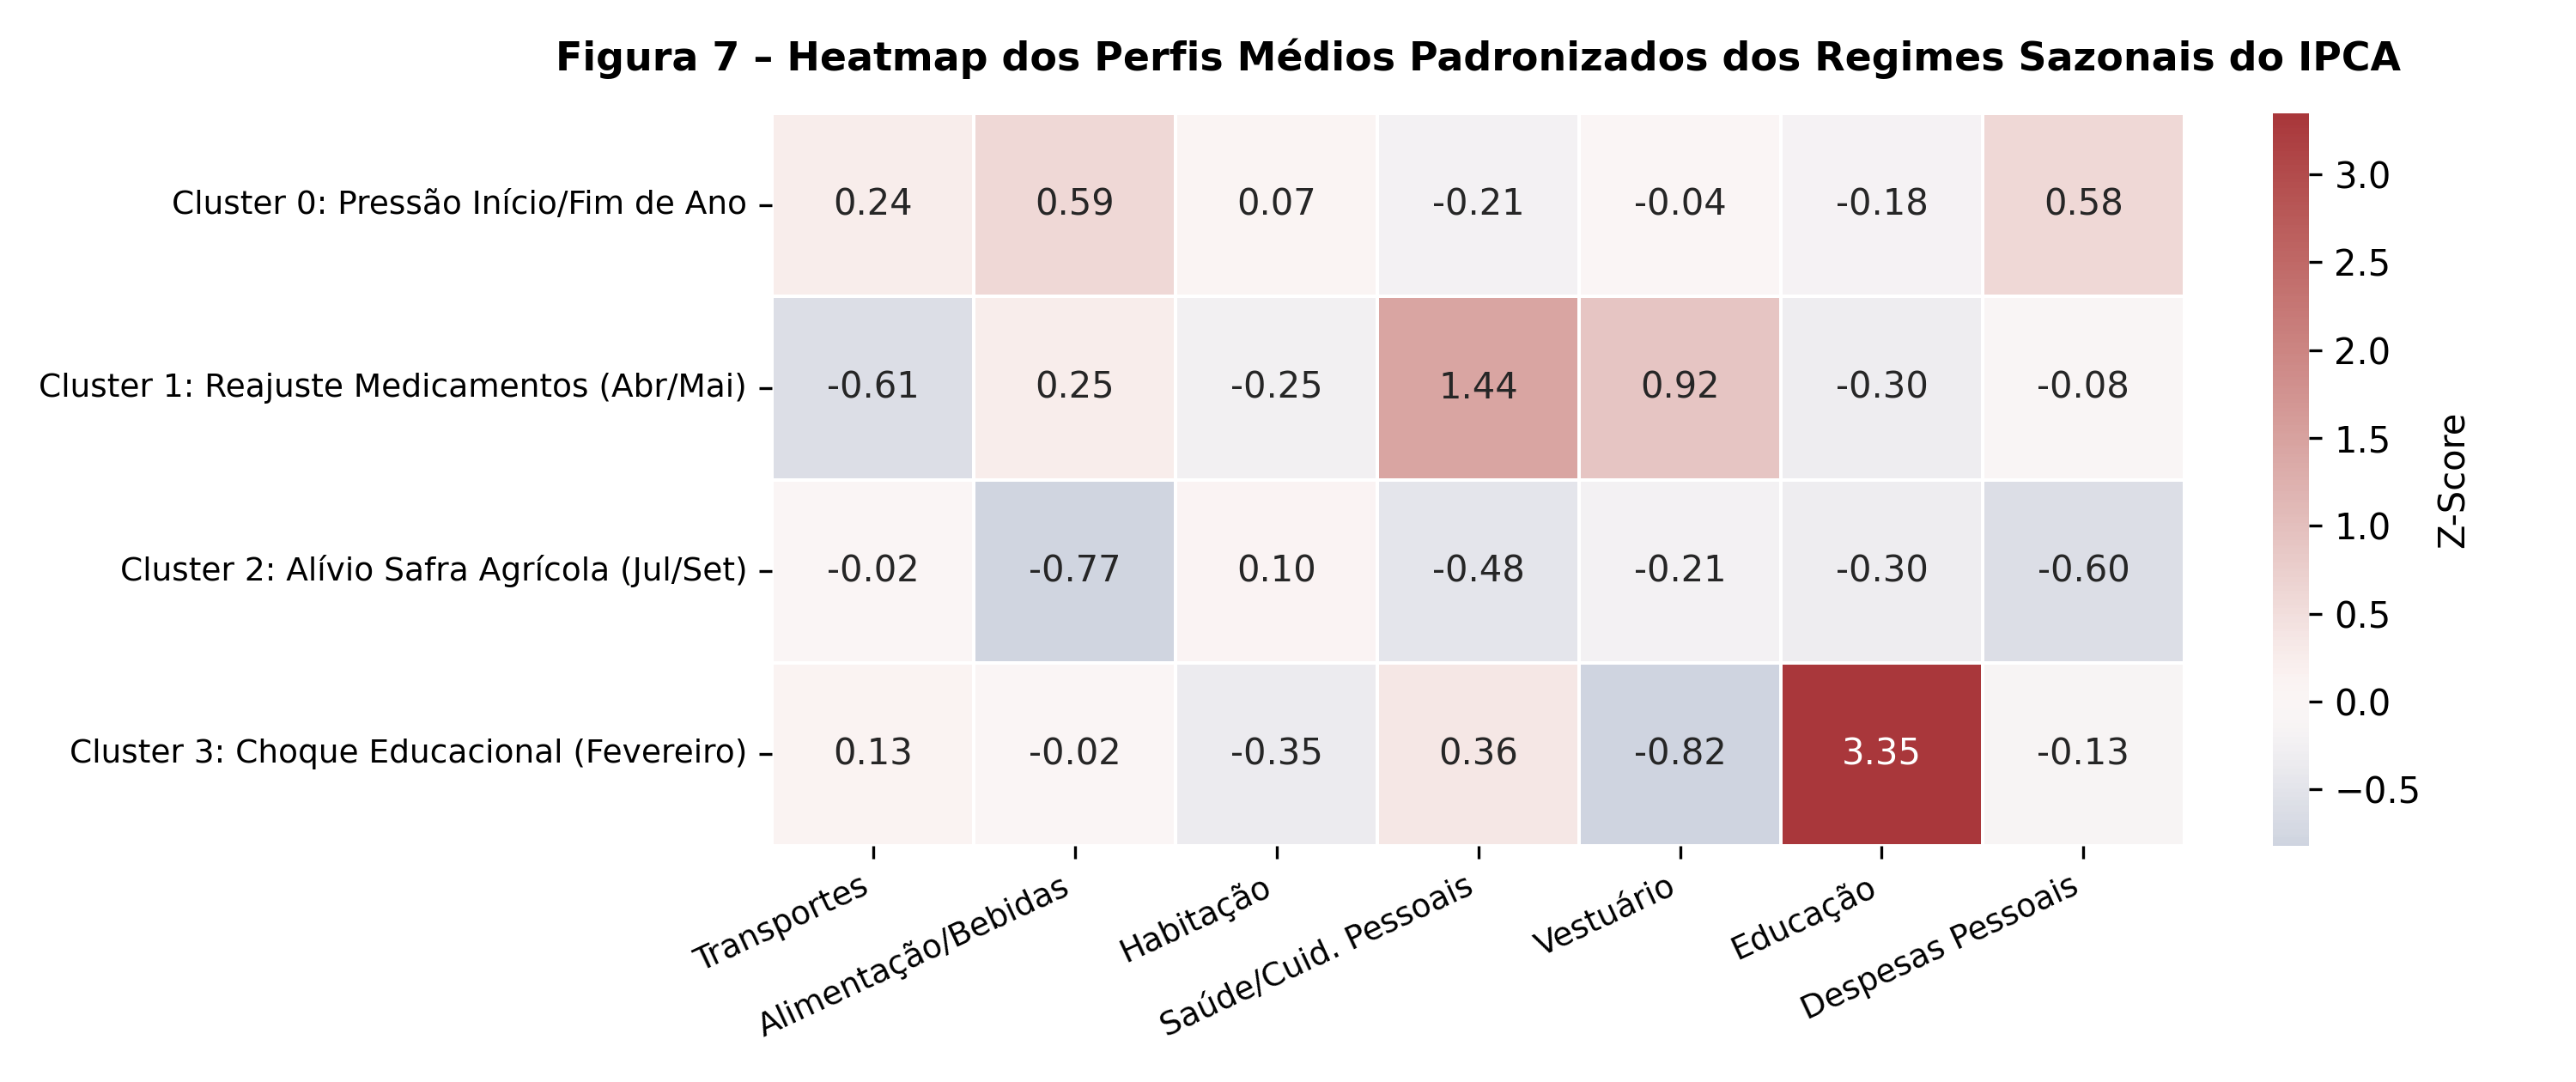
\includegraphics[width=0.88\linewidth]{Figura_7_Heatmap_Perfis_Sazonais.png}
\caption{Perfis Médios Padronizados ($Z$-Score) dos 7 Subcomponentes do IPCA nos 4 Regimes Sazonais.}
\label{fig:heat_sazonal}
\end{figure}

A caracterização econômica dos 4 regimes sazonais confirma as regularidades institucionais:
\begin{enumerate}
    \item \textbf{Cluster 3 -- Choque Educacional (Fevereiro):} Isola 12 dos 13 meses de fevereiro da série (92,3\% de especificidade), com desvio extremo em Educação ($+3,22\sigma$), refletindo reajustes de matrículas e mensalidades;
    \item \textbf{Cluster 1 -- Janela Regulatória de Medicamentos (Abril/Maio):} Concentra 13 dos 15 meses de abril, com desvio em Saúde e Cuidados Pessoais ($+1,15\sigma$), capturando o reajuste anual da CMED/ANVISA;
    \item \textbf{Cluster 2 -- Alívio de Safra Agrícola (Julho a Outubro):} Agrupa o período de colheita e clima seco, com forte deflação em Alimentação e Bebidas ($-0,58\sigma$);
    \item \textbf{Cluster 0 -- Pressões de Início e Fim de Ano (Novembro a Março):} Agrupa meses com pressões combinadas de demanda (13º salário, comércio, turismo) e reajustes tarifários municipais (transporte urbano).
\end{enumerate}

\paragraph{Conclusão da Camada 1: Reconstrução Não Supervisionada do Calendário Institucional}
O algoritmo de Ward reconstruiu autonomamente o calendário agrícola e regulatório brasileiro sem receber rótulos de data. O grupo Educação apresenta média histórica de +0,52\% ao mês e salta para impressionantes \textbf{+5,12\% ao mês} em Fevereiro ($Z$-Score médio de \textbf{+3,34 desvios-padrão}), com sobreposição nula frente aos demais meses (mínimo de +3,53\% em fevereiro, valor nunca atingido no restante do ano). A distância euclidiana ao quadrado de 12,89 pontos na dimensão educacional explica por que o Ramo Laranja se isola na altura máxima da árvore hierárquica (distância 17,6).

\subsubsection{Camada 2: Regimes Macroeconômicos com Ouro e Taxa de Juros}
O agrupamento tridimensional $[\text{IPCA}_t, \Delta\text{SELIC}_t, \Delta\%\text{Ouro}_{BRL,t}]$ isolou 4 regimes macroeconômicos alinhados à teoria monetária, sintetizados na Tabela \ref{tab:perfis_macro}.

\begin{table}[H]
\centering
\caption{Caracterização Macroeconômica dos 4 Regimes Identificados por Ward ($N = 173$ meses)}
\label{tab:perfis_macro}
\footnotesize
\begin{tabular}{lcccccc}
\toprule
\textbf{Regime Macroeconômico} & \textbf{Meses} & \textbf{IPCA (\%)} & \textbf{$\Delta$SELIC (p.p.)} & \textbf{Ret. Ouro (\%)} & \textbf{Juro Real (\%)} & \textbf{Câmbio} \\
\midrule
\textbf{0: Aperto Hawkish} & 53 & 0,501\% & \textbf{+0,064} & -3,318\% & +0,327\% & 3,896 \\
\textbf{1: Voo p/ Qualidade} & 67 & 0,283\% & -0,026 & \textbf{+5,220\%} & +0,465\% & 4,157 \\
\textbf{2: Desinflação/Cortes} & 23 & \textbf{-0,067\%} & \textbf{-0,117} & -1,014\% & \textbf{+0,927\%} & 3,968 \\
\textbf{3: Choque Severo} & 30 & \textbf{1,044\%} & +0,045 & \textbf{+2,368\%} & \textbf{-0,328\%} & \textbf{4,375} \\
\bottomrule
\end{tabular}
\end{table}

A dispersão bivariada dos 4 regimes é ilustrada na Figura \ref{fig:macro_scatter}.

\begin{figure}[H]
\centering
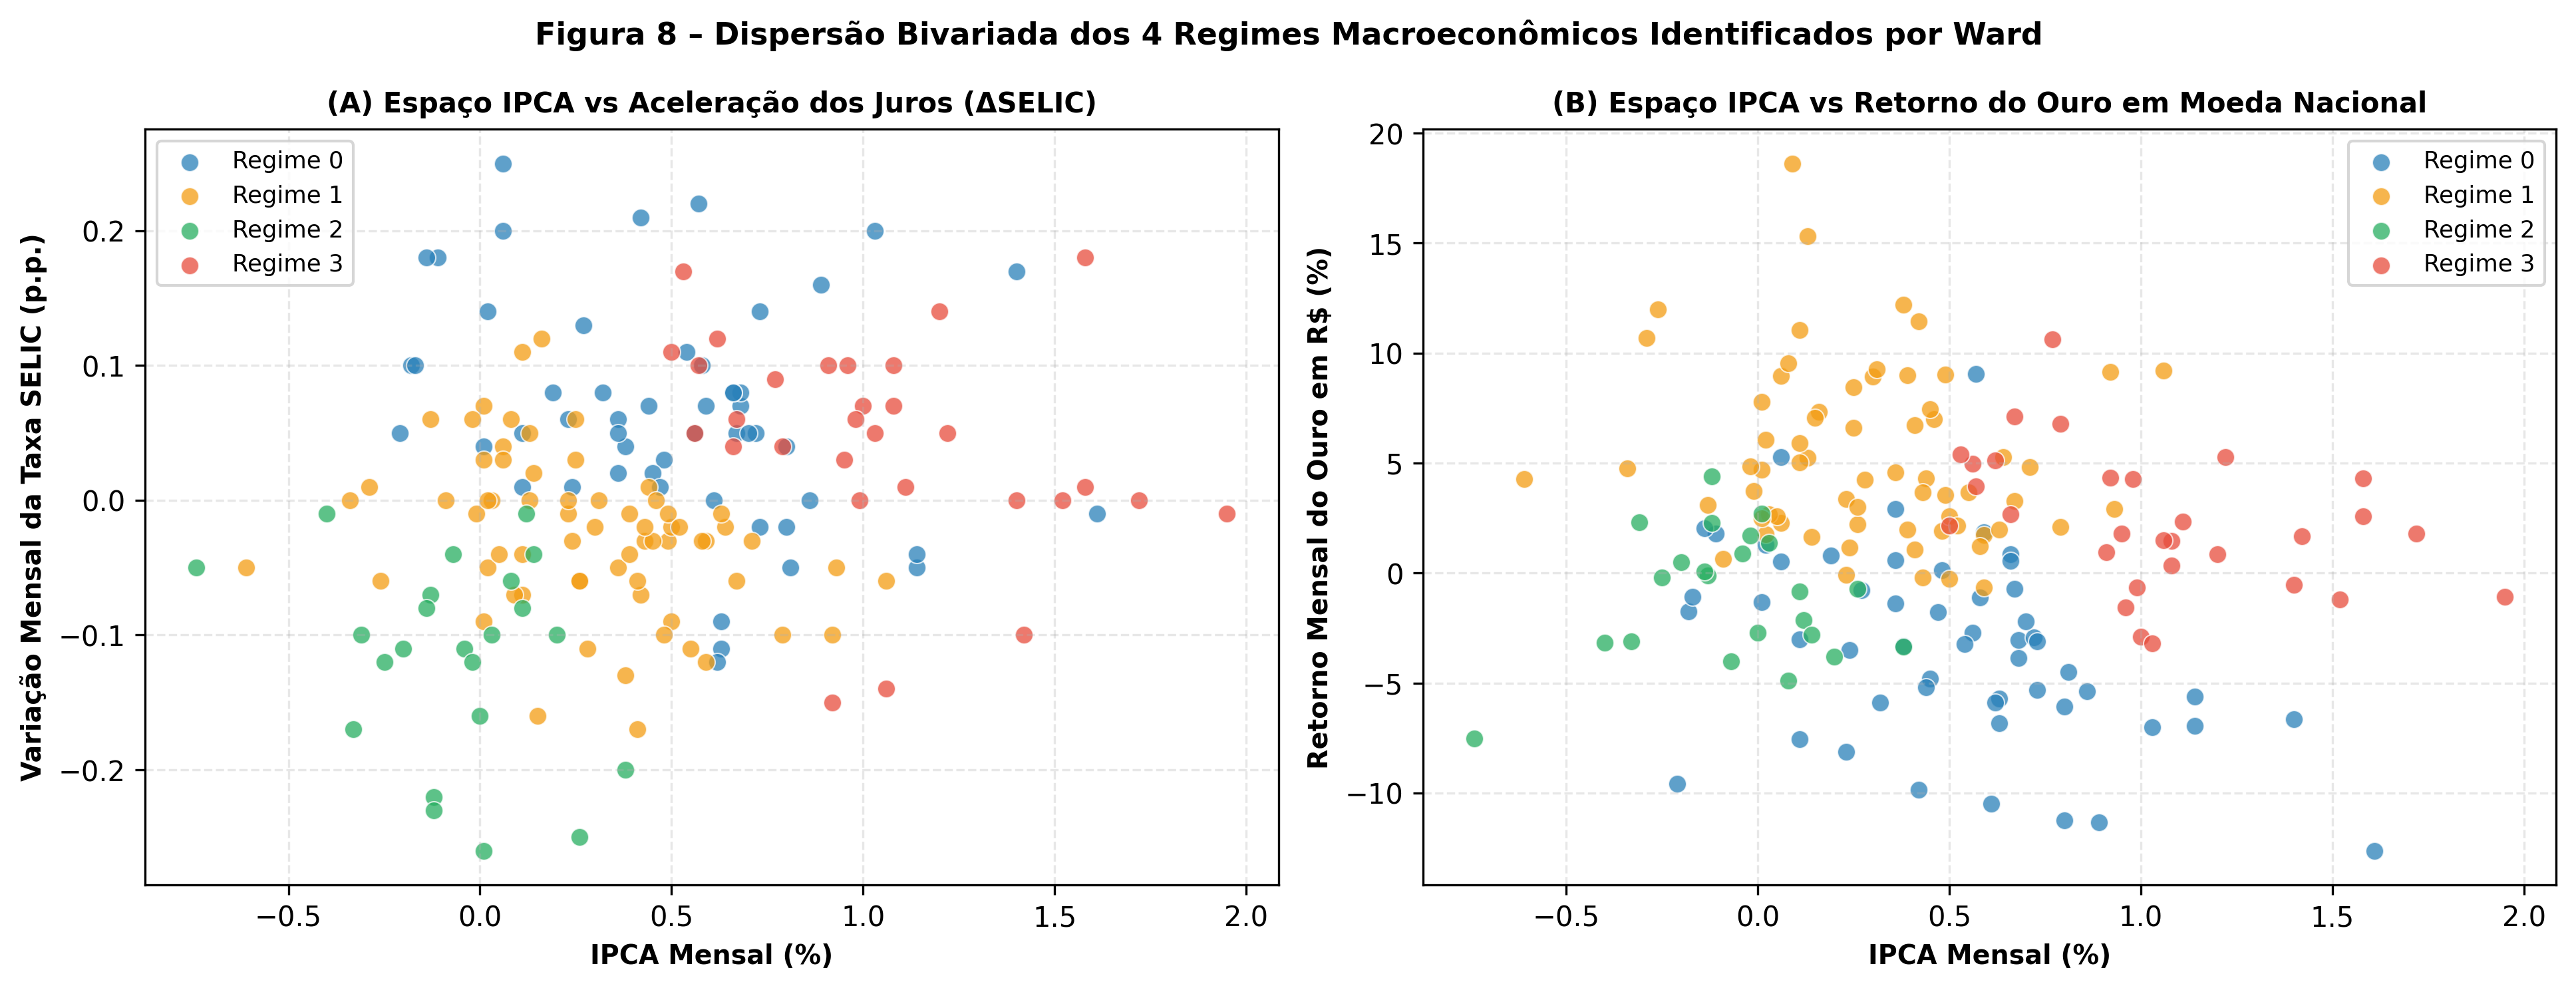
\includegraphics[width=0.98\linewidth]{Figura_8_Clusters_Macro_Ouro_Juros.png}
\caption{Dispersão Bivariada dos 4 Regimes Macroeconômicos: (A) IPCA vs $\Delta$SELIC; (B) IPCA vs Retorno do Ouro em Reais.}
\label{fig:macro_scatter}
\end{figure}

\paragraph{Conclusão da Camada 2: Não Linearidade da Trinca Inflação-Juros-Ouro e Identificação de Regimes}
O agrupamento tridimensional revela que Ouro e Selic operam como forças opostas no Brasil: no Regime 0 (Aperto Hawkish), a elevação de juros ($\Delta\text{SELIC} = +0,064$ p.p.) induz contração média de \textbf{-3,32\% no ouro em Reais}. No Regime 1 (Voo para Qualidade), o ouro dispara \textbf{+5,22\% ao mês} em resposta a tensões cambiais antes do repasse aos preços. No Regime 2 (Desinflação Dovish), a deflação ($-0,067\%$) associada à queda de juros eleva o \textbf{Juro Real ao recorde histórico de +0,93\% ao mês}. Por fim, o Regime 3 (Choque Severo, IPCA de +1,04\%) flagra a política monetária defasada, empurrando o juro real para o campo negativo ($-0,33\%$) e estimulando a fuga para o ouro (+2,37\%).

\subsubsection{Camada 3: Interação Cruzada e Teste de Independência}
A matriz de contingência da Figura \ref{fig:contingencia} cruza as partições da Camada 1 e Camada 2.

\begin{figure}[H]
\centering
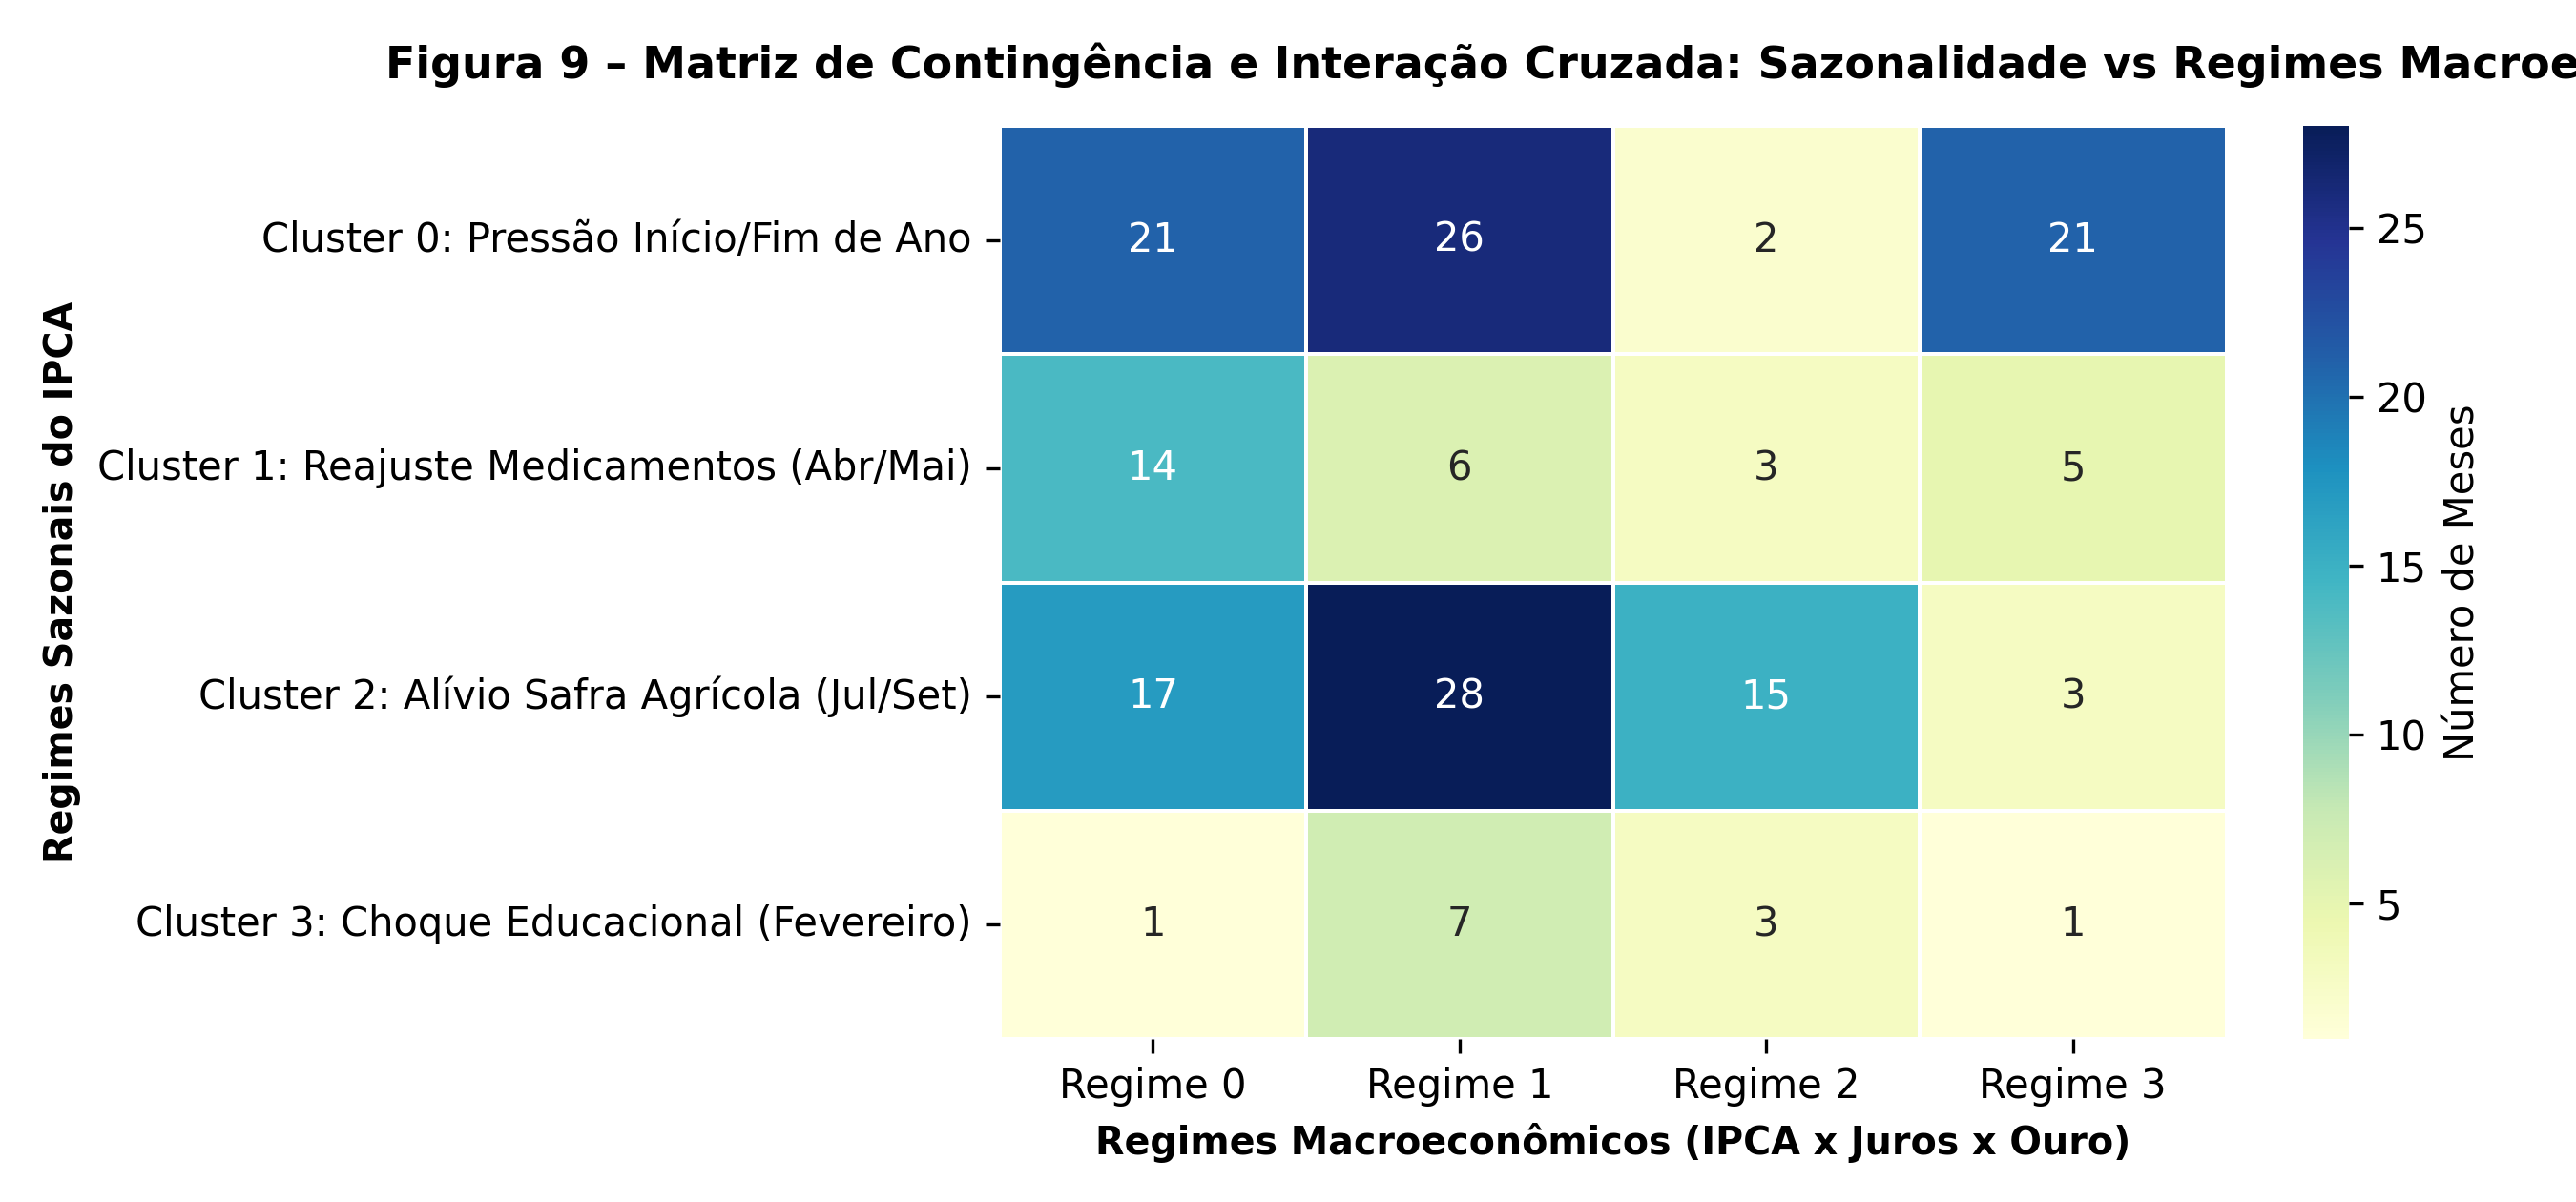
\includegraphics[width=0.88\linewidth]{Figura_9_Matriz_Contingencia_Sazonal_Macro.png}
\caption{Matriz de Contingência e Interação Cruzada: Regimes Sazonais vs Regimes Macroeconômicos.}
\label{fig:contingencia}
\end{figure}

O Teste Qui-Quadrado de Pearson resultou em $\chi^2 = 34{,}82$ ($p = 0{,}0001$), rejeitando a independência. Evidencia-se que 65,2\% dos meses de desinflação ocorrem na safra agrícola, enquanto o Choque Inflacionário Severo suprime o alívio de safra (apenas 3 ocorrências).

\paragraph{Conclusão da Camada 3: Rejeição da Independência e Modulação Macroeconômica da Safra}
O Teste Qui-Quadrado de Pearson ($\chi^2 = 34,73, p = 0,000067$) refuta a independência entre sazonalidade e choques macroeconômicos. Evidencia-se que \textbf{65,2\% dos episódios de afrouxamento monetário sustentado (Regime 2)} dependem da descompressão de preços da Safra Agrícola de inverno. Em contrapartida, sob Choques Inflacionários Severos (Regime 3), a safra é anulada (apenas 10\% de incidência), demonstrando que pressões externas severas de custos e ouro suprimem o alívio sazonal biológico dos alimentos.

\subsection{Considerações Finais e Trabalhos Futuros}

% =====================================================================

O presente estudo estruturou com rigor metodológico o \textit{pipeline} de dados para o enfrentamento de um dos mais desafiadores problemas econométricos da economia brasileira: a modelagem e previsão do IPCA. Ao longo de 174 meses contínuos (2012–2026), articulou-se a coleta automatizada de 29 variáveis macroeconômicas oficiais, estabelecendo rotinas robustas de higienização, tratamento de zeros contábeis e imputação causal temporal estrita, imune a vazamentos preditivos (\textit{zero data leakage}).

A análise exploratória descritiva comprovou as propriedades teóricas da série: a presença de assimetria positiva (+0,53) e caudas pesadas com cinco \textit{outliers} históricos acentuados evidencia que a inflação brasileira não pode ser modelada sob premissas gaussianas estritas. Além disso, a categorização em regimes nominais revelou que mais de 40\% das observações operaram acima do teto estipulado pelas autoridades monetárias, ratificando a relevância de variáveis de pressão externa (como o câmbio PTAX e combustíveis) para a antecipação de mudanças de regime.

Como desdobramentos imediatos para a próxima etapa do projeto, delineiam-se:
\begin{enumerate}[leftmargin=1.5em]
    \item A implementação dos algoritmos bioinspirados de seleção de atributos (Algoritmos Genéticos e PSO) para identificar a combinação parcimoniosa ótima de variáveis exógenas e defasagens temporais \cite{ref8, ref11};
    \item A calibração da arquitetura híbrida de previsão: um componente linear ARIMAX para absorver a inércia autorregressiva estocástica, acoplado a um regressor \textit{Random Forest} responsável por capturar as interações não lineares sobre os resíduos \cite{ref14, ref18};
    \item A avaliação comparativa de acurácia através de janelas temporais deslizantes (\textit{rolling windows}) de 1 a 12 meses à frente frente aos \textit{benchmarks} econométricos clássicos \cite{ref6, ref9}.
\end{enumerate}

% =====================================================================
% REFERÊNCIAS BIBLIOGRÁFICAS
% =====================================================================

\begin{thebibliography}{99}

\bibitem{ref1} BOX, G. E.; JENKINS, G. M.; REINSEL, G. C.; LJUNG, G. M. \textbf{Time Series Analysis: Forecasting and Control}. 5. ed. Hoboken: John Wiley \& Sons, 2015.

\bibitem{ref2} BANCO CENTRAL DO BRASIL (BACEN). \textbf{Sistema Gerenciador de Séries Temporais (SGS)}. Brasília: BACEN, 2026. Disponível em: <\url{https://www3.bcb.gov.br/sgspub/}>. Acesso em: 16 set. 2026.

\bibitem{ref3} BANCO CENTRAL DO BRASIL (BACEN). \textbf{Relatório de Inflação}, v. 26, n. 2. Brasília: Banco Central do Brasil, 2024.

\bibitem{ref4} BLANCHARD, O. \textbf{Macroeconomia}. 7. ed. São Paulo: Pearson, 2017.

\bibitem{ref5} BRESSER-PEREIRA, L. C.; NAKANO, Y. \textbf{A Teoria da Inflação Inercial}. São Paulo: Brasiliense, 1984.

\bibitem{ref6} GARCIA, M. G.; MEDEIROS, M. C.; VASCONCELOS, G. F. Real-time inflation forecasting with high-dimensional data: the case of Brazil. \textbf{International Journal of Forecasting}, v. 33, n. 3, p. 679–693, 2017.

\bibitem{ref7} HASTIE, T.; TIBSHIRANI, R.; FRIEDMAN, J. \textbf{The Elements of Statistical Learning: Data Mining, Inference, and Prediction}. 2. ed. New York: Springer, 2009.

\bibitem{ref8} HOLLAND, J. H. \textbf{Adaptation in Natural and Artificial Systems}. Cambridge: MIT Press, 1992.

\bibitem{ref9} HYNDMAN, R. J.; ATHANASOPOULOS, G. \textbf{Forecasting: Principles and Practice}. 3. ed. Melbourne: OTexts, 2021.

\bibitem{ref10} INSTITUTO BRASILEIRO DE GEOGRAFIA E ESTATÍSTICA (IBGE). \textbf{Sistema Nacional de Índices de Preços ao Consumidor (SNIPC): Metodologia do IPCA e INPC}. Rio de Janeiro: IBGE, 2020.

\bibitem{ref11} KENNEDY, J.; EBERHART, R. Particle swarm optimization. In: \textbf{Proceedings of ICNN'95 - IEEE International Conference on Neural Networks}, v. 4, p. 1942–1948, 1995.

\bibitem{ref12} KHANDANI, A. E.; KIM, A. J.; LO, A. W. Consumer credit-risk models via machine-learning algorithms. \textbf{Journal of Banking \& Finance}, v. 34, n. 11, p. 2767–2787, 2010.

\bibitem{ref13} MANKIW, N. G. \textbf{Macroeconomia}. 10. ed. Rio de Janeiro: LTC, 2021.

\bibitem{ref14} MEDEIROS, M. C.; VASCONCELOS, G. F.; VEIGA, Á.; ZILBERMAN, E. Forecasting inflation in a data-rich environment: the benefits of machine learning methods. \textbf{Journal of Business \& Economic Statistics}, v. 39, n. 1, p. 98–119, 2021.

\bibitem{ref15} PEDREGOSA, F. et al. Scikit-learn: Machine Learning in Python. \textbf{Journal of Machine Learning Research}, v. 12, p. 2825–2830, 2011.

\bibitem{ref16} SIMONSEN, M. H. \textbf{30 Anos de Indexação}. Rio de Janeiro: Editora FGV, 1995.

\bibitem{ref17} TAYLOR, J. B. Discretion versus policy rules in practice. \textbf{Carnegie-Rochester Conference Series on Public Policy}, v. 39, p. 195–214, 1993.

\bibitem{ref18} ZHANG, G. P. Time series forecasting using a hybrid ARIMA and neural network model. \textbf{Neurocomputing}, v. 50, p. 159–175, 2003.

\bibitem{ref19} WARD, J. H. Hierarchical grouping to optimize an objective function. \textbf{Journal of the American Statistical Association}, v. 58, n. 301, p. 236--244, 1963.
\bibitem{ref20} LANCE, G. N.; WILLIAMS, W. T. A general theory of classificatory sorting strategies: II. Clustering systems. \textbf{The Computer Journal}, v. 10, n. 3, p. 271--277, 1967.
\bibitem{ref21} BAUR, D. G.; LUCEY, B. M. Is gold a hedge or a safe haven? An analysis of stocks, bonds and gold. \textbf{Financial Review}, v. 45, n. 2, p. 217--229, 2010.
\bibitem{ref22} ERB, C. B.; HARVEY, C. R. The golden dilemma. \textbf{Financial Analysts Journal}, v. 69, n. 4, p. 10--42, 2013.

\end{thebibliography}

\end{document}